\documentclass[10pt,openany]{book}
\usepackage[utf8]{inputenc}
\DeclareUnicodeCharacter{2212}{\ensuremath{-}}
\DeclareUnicodeCharacter{2192}{\ensuremath{\to}}
\DeclareUnicodeCharacter{03B1}{\ensuremath{\alpha}}
\usepackage[T1]{fontenc}
\usepackage{lmodern}
\AtBeginDocument{\normalfont\DeclareFontShape{T1}{lmr}{bx}{sc}{<->ssub*lmr/m/sc}{}}
\usepackage[spanish,es-nodecimaldot]{babel}
\spanishplainpercent
\AtBeginDocument{\spanishdeactivate{"~<>}}
\usepackage[a4paper,margin=2.5cm,headheight=14pt]{geometry}
\usepackage{amsmath,amssymb,mathtools,booktabs,array,longtable,graphicx,xcolor,tikz,enumitem,microtype,titlesec,fancyhdr}
\usepackage[breakable,skins]{tcolorbox}
\usepackage[labelfont=bf]{caption}
\usepackage[hyphens]{url}
\usepackage[hidelinks,unicode,hypertexnames=false]{hyperref}
\definecolor{studiumInk}{RGB}{20,44,64}
\definecolor{studiumBlue}{RGB}{24,74,130}
\definecolor{studiumCyan}{RGB}{0,184,205}
\definecolor{studiumLight}{RGB}{232,240,250}
\definecolor{studiumWorkedBack}{RGB}{255,244,230}
\definecolor{studiumWorkedFrame}{RGB}{138,78,12}
\definecolor{studiumCheckBack}{RGB}{243,236,248}
\definecolor{studiumCheckFrame}{RGB}{96,48,130}
\titleformat{\chapter}[display]{\normalfont\filright}{\large\mdseries\scshape\chaptertitlename\ \thechapter}{1ex}{\normalfont\huge\bfseries}
\titlespacing*{\chapter}{0pt}{2.5ex plus 1ex minus .2ex}{2.3ex}
\titleformat{name=\chapter,numberless}[display]{\normalfont\filright}{}{0pt}{\normalfont\huge\bfseries}
\titleformat{\section}{\Large\bfseries}{\thesection}{.8em}{}
\titleformat{\subsection}{\large\bfseries}{\thesubsection}{.7em}{}
\makeatletter
\renewcommand*\l@section{\@dottedtocline{1}{1.5em}{3.5em}}
\makeatother
\setcounter{secnumdepth}{2}\setcounter{tocdepth}{1}
\setlength{\parindent}{1.5em}\setlength{\parskip}{3pt plus .5pt}
\setlength{\emergencystretch}{1.5em}\raggedbottom
\setlist{itemsep=2pt,topsep=4pt,leftmargin=*}
\setlist[description]{style=nextline,leftmargin=0pt,labelwidth=0pt,labelindent=0pt}
\allowdisplaybreaks[2]
\graphicspath{{../figures/}}
\newcommand{\Raire}{287.05287}
\newcommand{\gzero}{9.80665}
\tcbset{studiumcommon/.style={breakable,boxrule=.65pt,arc=.7pt,left=1.7mm,right=1.7mm,top=1.3mm,bottom=1.3mm,before skip=10pt,after skip=10pt,fonttitle=\bfseries}}
\newtcolorbox{studiumworked}[1]{studiumcommon,colback=studiumWorkedBack,colframe=studiumWorkedFrame,colbacktitle=studiumWorkedFrame,coltitle=white,title={#1}}
\newcommand{\objetivos}[1]{\par\noindent\textbf{Objetivos de aprendizaje.} \textit{#1}\par\medskip}
\newcommand{\caja}[2]{\begin{tcolorbox}[studiumcommon,colback=studiumLight,colframe=studiumBlue,colbacktitle=studiumBlue,coltitle=white,title={#1}]#2\end{tcolorbox}}
\newcommand{\resumen}[1]{\begin{tcolorbox}[studiumcommon,colback=studiumCheckBack,colframe=studiumCheckFrame,colbacktitle=studiumCheckFrame,coltitle=white,title=Resumen]#1\end{tcolorbox}}
\newcommand{\figura}[2]{\begin{figure}[tbp]\centering\includegraphics[width=.83\linewidth]{#1.pdf}\caption{#2}\label{fig:#1}\end{figure}\noindent La figura~\ref{fig:#1} ofrece una representación del modelo discutido.}
\pagestyle{fancy}\fancyhf{}
\fancyhead[LE]{\small\thepage\hspace{1.5em}\mdseries\scshape\nouppercase{\leftmark}}
\fancyhead[RO]{\small\mdseries\scshape\nouppercase{\rightmark}\hspace{1.5em}\thepage}
\renewcommand{\headrulewidth}{.4pt}\renewcommand{\footrulewidth}{0pt}
\fancypagestyle{plain}{\fancyhf{}\fancyfoot[C]{\small\thepage}\renewcommand{\headrulewidth}{0pt}}
\newcommand{\portada}[2]{\hypersetup{pageanchor=false}\begin{titlepage}\thispagestyle{empty}
\begin{tikzpicture}[remember picture,overlay,x=1pt,y=-1pt]
\begin{scope}[shift={(current page.north west)}]
\clip (0,0) rectangle (595.276,841.89);
\node[inner sep=0pt] at (297.638,420.945){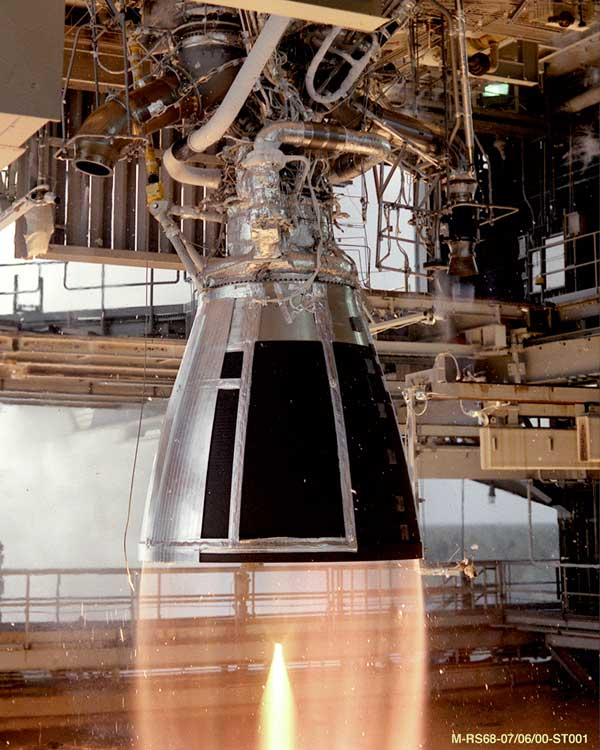
\includegraphics[height=\paperheight]{RS-68_rocket_engine_test.jpg}};
\fill[white,opacity=.91] (0,0) rectangle (595.276,89.5);
\fill[studiumInk,opacity=.96] (0,585.5) rectangle (595.276,841.89);
\node[anchor=west,text=studiumInk,font=\sffamily\bfseries\fontsize{18}{20}\selectfont,inner sep=0pt] at (51.223,38.5){STUDIUM};
\fill[studiumCyan] (51.223,61.5) rectangle (80.8,63.7);
\node[anchor=west,text=studiumInk,font=\sffamily\fontsize{9}{11}\selectfont,inner sep=0pt] at (89.49,65.5){BIBLIOTECA DE INGENIERÍA};
\node[anchor=west,text=studiumCyan,font=\sffamily\bfseries\fontsize{10}{12}\selectfont,inner sep=0pt] at (51.223,608){MANUAL UNIVERSITARIO};
\node[anchor=north west,text=white,text width=493pt,font=\rmfamily\bfseries\fontsize{33}{36}\selectfont,inner sep=0pt] at (51.223,636){#1};
\node[anchor=west,text=white!82!studiumInk,font=\sffamily\fontsize{11}{14}\selectfont,inner sep=0pt] at (51.223,732){#2};
\node[anchor=west,text=white,font=\sffamily\bfseries\fontsize{10}{12}\selectfont,inner sep=0pt] at (51.223,758){GRADO EN INGENIERÍA AEROESPACIAL};
\node[anchor=west,text=white!82!studiumInk,font=\sffamily\fontsize{10}{12}\selectfont,inner sep=0pt] at (51.223,773){Universidad de León};
\draw[white!75!studiumInk,line width=.4pt] (51.223,786) -- (544.05,786);
\node[anchor=west,text=white!82!studiumInk,font=\sffamily\fontsize{10}{12}\selectfont,inner sep=0pt] at (51.223,810){2026};
\node[anchor=east,text=white,font=\sffamily\bfseries\fontsize{10}{12}\selectfont,inner sep=0pt] at (544.05,810){I Edición};
\end{scope}\end{tikzpicture}\null\end{titlepage}\hypersetup{pageanchor=true}}

\hypersetup{pdftitle={PROBLEMAS RESUELTOS DE MOTORES COHETE},pdfauthor={Daniel Miguel Tejedor}}
\renewcommand{\studiumvolumetype}{problemas}
\begin{document}
\studiumcover{MOTORES COHETE}{Problemas resueltos y comprobaciones}{PROBLEMAS RESUELTOS}
\frontmatter
\studiumreadingguide
\chapter*{Presentación y alcance}
\addcontentsline{toc}{chapter}{Presentación y alcance}
Este volumen pertenece al proyecto independiente de Motores Cohete, Universidad de León, curso 2026/2027. Es una elaboración original de apoyo al estudio, sin atribución de autoría ni aval a la Universidad. Los controles ejecutados y su alcance se detallan en los informes, junto con las comprobaciones pendientes.

La estructura académica conserva los seis bloques de la guía oficial. Los 28 capítulos, los problemas y los simulacros son decisiones editoriales. Los documentos proporcionados se abrieron y contrastaron; los manuscritos estudiantiles se usan para analizar competencias y posibles errores, sin copiar páginas, figuras ni enunciados extensos.

Los modelos se acompañan de hipótesis y límites. La reproducción aritmética, el álgebra simbólica, las dimensiones, la conservación y la validación experimental son niveles diferentes. Una solución de equilibrio o una curva ideal no se presenta como un ensayo real.

La procedencia técnica y los controles ejecutados se conservan en el repositorio del libro.

Se adopta $g_0=9.80665\,\mathrm{m/s^2}$ y unidades SI. Los decimales adicionales de algunas soluciones facilitan comprobar cálculos; no representan precisión experimental. Los niveles básico, intermedio, avanzado y de examen son orientativos.

Este cuaderno añade 36 problemas con datos nuevos. Los niveles son orientativos y no reproducen exámenes oficiales. Se recomienda intentar cada enunciado antes de leer su desarrollo; las comprobaciones explicitan qué se ha conservado y qué queda fuera del modelo.
\tableofcontents
\mainmatter
\chapter{Bloque 1. Introducción y fundamentos}
\section{P01. Momento y presión en dos ambientes}
\begin{studiumworked}{P01. Momento y presión en dos ambientes · Básico}
\textbf{Enunciado.} Una descarga académica uniforme tiene caudal $1.99\,\mathrm{kg/s}$, rapidez $2281\,\mathrm{m/s}$, presión de salida $43\,\mathrm{kPa}$ y área $0.0096\,\mathrm{m^2}$. El ambiente tiene $79\,\mathrm{kPa}$. Determine empuje, velocidad efectiva e impulso específico, y repita para vacío conservando el estado interno.

\textbf{Datos.} Caudal total: $1.99\,\mathrm{kg/s}$; Rapidez axial: $2281\,\mathrm{m/s}$; Salida: $43000\,\mathrm{Pa}$; Ambiente: $79000\,\mathrm{Pa}$; Área de salida: $0.0096\,\mathrm{m^2}$.

\textbf{Incógnitas.} F, c, Isp y cambio a vacío.

\textbf{Hipótesis.} Estacionario, axial y salida uniforme. Estado interno invariable y flujo adherido supuesto; no se prueba su régimen con los datos disponibles.

\textbf{Modelo físico.} Balance de momento respecto al ambiente.
\[F=\dot m v_e+(p_e-p_a)A_e\]
\[c=F/\dot m,\quad I_{sp}=c/g_0\]
\[F_v-F=p_aA_e\]
\textbf{Desarrollo.}
\begin{enumerate}
\item La contribución cinética es $1.99$ por $2281$, igual a $4539.19\,\mathrm{N}$. La presión aporta $(43000-79000)0.0096=-345.6$ N.
\item Sumar ambas da $4193.59\,\mathrm{N}$. Dividir por $1.99\,\mathrm{kg/s}$ produce $2107.332\,\mathrm{m/s}$; dividir después por $g_0$ produce $214.888\,\mathrm{s}$.
\item En vacío se conserva la descarga y se elimina únicamente $-p_aA_e$. Resulta $4951.99\,\mathrm{N}$, con $253.75\,\mathrm{s}$. No se impone adaptación para efectuar ninguno de los dos cálculos.
\end{enumerate}
\textbf{Operaciones para contrastar el cálculo.}
\begin{enumerate}

\item Magnitud 1.

\[\fitmath{y_{1}=1.99\cdot 2281+\left(43000-79000\right)\cdot 0.0096\approx 4193.59\,\mathrm{N}}\]

\item Magnitud 2.

\[\fitmath{y_{2}=\frac{4193.59}{1.99\cdot 9.80665}\approx 214.888\,\mathrm{s}}\]

\end{enumerate}

\textbf{Resultados.} $F=4193.59$ N; $c=2107.332$ m/s; $I_{sp}=214.888$ s; $F_v=4951.99$ N.

\textbf{Interpretación.} La rapidez física permanece fija, pero el impulso específico cambia con el ambiente porque incluye el empuje de presión. Un cociente de presiones no se deduce de haber calculado un empuje positivo.

\textbf{Comprobación.} La diferencia a vacío es $758.4\,\mathrm{N}$ y coincide con $p_aA_e$. Recuperar $g_0I_{sp}$ debe dar $F/\dot m$, no necesariamente $v_e$.

\textbf{Límites.} No se han establecido dimensiones de garganta ni un mapa de régimen; no es una predicción de separación ni de estabilidad de un motor.
\end{studiumworked}
\section{P02. Dos rutas para la velocidad de una expansión}
\begin{studiumworked}{P02. Dos rutas para la velocidad de una expansión · Básico}
\textbf{Enunciado.} Un gas académico de $\gamma=1.3$ y masa molar $23.4\,\mathrm{kg/kmol}$ tiene $T_0=2440$ K y $p_0=2.50$ MPa. Una sección isentrópica alcanza $M=2.1$. Halle $R,c_p,T,p,u$ y verifique energía.

\textbf{Datos.} Exponente constante: $1.3$; Masa molar: $23.4\,\mathrm{kg/kmol}$; Temperatura total: $2440\,\mathrm{K}$; Presión total: $2.500000\times10^{6}\,\mathrm{Pa}$; Mach: $2.1$.

\textbf{Incógnitas.} Propiedades específicas y estado estático.

\textbf{Hipótesis.} Gas caloríficamente perfecto de composición fija. Expansión adiabática reversible, sin trabajo ni altura.

\textbf{Modelo físico.} Energía y relaciones de remanso.
\[R=R_u/\mathcal M,\quad c_p=\gamma R/(\gamma-1)\]
\[T=T_0/[1+(\gamma-1)M^2/2]\]
\[p=p_0(T/T_0)^{\gamma/(\gamma-1)}\]
\[u=M\sqrt{\gamma RT}=\sqrt{2c_p(T_0-T)}\]
\textbf{Desarrollo.}
\begin{enumerate}
\item Se usa $R_u=8314.462618$ J/(kmol K), coherente con kg/kmol. Así $R=355.3189$ J/(kg K) y $c_p=1539.715$ J/(kg K).
\item El factor de remanso es $1.6615$. Dividir $T_0$ da $1468.553\,\mathrm{K}$; la potencia isentrópica da $276.9737\,\mathrm{kPa}$.
\item Con la temperatura estática, la ruta acústica da $1729.597\,\mathrm{m/s}$. La ruta energética usa el descenso $c_p(T_0-T)$ y produce el mismo valor. Usar $T_0$ dentro del sonido de la sección daría otra rapidez incompatible.
\end{enumerate}
\textbf{Operaciones para contrastar el cálculo.}
\begin{enumerate}

\item Magnitud 1.

\[\fitmath{y_{1}=\frac{8314.462618}{23.4}\approx 355.3189\,\mathrm{J/(kg\,K)}}\]

\item Magnitud 2.

\[\fitmath{y_{2}=2.1\cdot \sqrt{1.3\cdot 355.3189153\cdot 1468.552513}\approx 1729.597\,\mathrm{m/s}}\]

\item Magnitud 3.

\[\fitmath{y_{3}=1539.7153\cdot 1468.552513+\frac{{1729.596808}^{2}}{2}\approx 3756905\,\mathrm{J/kg}}\]

\end{enumerate}

\textbf{Resultados.} $T=1468.553$ K; $p=2.769737\times10^{5}$ Pa; $u=1729.597$ m/s.

\textbf{Interpretación.} El gas acelera y enfría, pero su temperatura total permanece fija. La presión total se mantiene sólo porque se ha supuesto isentropía.

\textbf{Comprobación.} $c_pT+u^2/2=c_pT_0=3.756905\times10^{6}$ J/kg. La entropía calculada mediante $c_p\ln(T/T_0)-R\ln(p/p_0)$ es cero dentro de redondeo.

\textbf{Límites.} No se modela química ni variación calorífica; gamma es un dato académico, no una propiedad universal de productos reales.
\end{studiumworked}
\section{P03. Incertidumbre de un cociente correlacionado}
\begin{studiumworked}{P03. Incertidumbre de un cociente correlacionado · Intermedio}
\textbf{Enunciado.} Se miden $F=4250$ N y $\dot m=1.8$ kg/s. Sus incertidumbres estándar relativas son $1.1$\,\% y 0.7\,\%, con correlación $r=0.25$. Estime $I_{sp}$ y su incertidumbre linealizada; compare con asumir independencia.

\textbf{Datos.} Empuje: $4250\,\mathrm{N}$; Caudal: $1.8\,\mathrm{kg/s}$; Incertidumbre relativa: $0.011$; Incertidumbre relativa: $0.007$; Correlación: $0.25$.

\textbf{Incógnitas.} Impulso específico e incertidumbre estándar.

\textbf{Hipótesis.} Perturbaciones pequeñas y modelo diferenciable. g0 convencional; correlación proporcionada.

\textbf{Modelo físico.} Propagación mediante gradiente y covarianza.
\[I_{sp}=F/(g_0\dot m)\]
\[(u_I/I_{sp})^2=u_F^2/F^2+u_m^2/\dot m^2-2r(u_F/F)(u_m/\dot m)\]
\textbf{Desarrollo.}
\begin{enumerate}
\item Las sensibilidades son $\partial I/\partial F=1/(g_0\dot m)$ y $\partial I/\partial\dot m=-F/(g_0\dot m^2)$. Sus signos opuestos explican el signo negativo de la covarianza.
\item La sustitución da $I_{sp}=240.7663$ s y $u_I/I_{sp}=\sqrt{0.011^2+0.007^2-2(0.25)(0.011)(0.007)}=0.01146734$.
\item Multiplicar por el valor central da $2.760951\,\mathrm{s}$. Si se impone $r=0$, la incertidumbre relativa sería $1.30384$\,\%; esa diferencia no es una mejora del sensor sino un cambio del modelo de correlación.
\end{enumerate}
\textbf{Operaciones para contrastar el cálculo.}
\begin{enumerate}

\item Magnitud 1.

\[\fitmath{y_{1}=\frac{4250}{1.8\cdot 9.80665}\approx 240.7663\,\mathrm{s}}\]

\item Magnitud 2.

\[\fitmath{y_{2}=\sqrt{{0.011}^{2}+{0.007}^{2}-2\cdot 0.25\cdot 0.011\cdot 0.007}\approx 0.01146734\,}\]

\end{enumerate}

\textbf{Resultados.} $I_{sp}=240.7663$ s; $u(I_{sp})=2.760951$ s.

\textbf{Interpretación.} Las variaciones comunes de empuje y caudal pueden compensarse parcialmente en su cociente. La incertidumbre instrumental no cuantifica por sí sola error de modelo físico.

\textbf{Comprobación.} La matriz de correlación es admisible porque $|r|\leq1$. El radicando es no negativo y el resultado conserva unidad de segundos.

\textbf{Límites.} No es un intervalo de confianza expandido; no se asigna cobertura sin una distribución y factor definidos.
\end{studiumworked}
\section{P04. Momento y presión en dos ambientes}
\begin{studiumworked}{P04. Momento y presión en dos ambientes · Intermedio}
\textbf{Enunciado.} Una descarga académica uniforme tiene caudal $2.38\,\mathrm{kg/s}$, rapidez $2362\,\mathrm{m/s}$, presión de salida $46\,\mathrm{kPa}$ y área $0.0102\,\mathrm{m^2}$. El ambiente tiene $76\,\mathrm{kPa}$. Determine empuje, velocidad efectiva e impulso específico, y repita para vacío conservando el estado interno.

\textbf{Datos.} Caudal total: $2.38\,\mathrm{kg/s}$; Rapidez axial: $2362\,\mathrm{m/s}$; Salida: $46000\,\mathrm{Pa}$; Ambiente: $76000\,\mathrm{Pa}$; Área de salida: $0.0102\,\mathrm{m^2}$.

\textbf{Incógnitas.} F, c, Isp y cambio a vacío.

\textbf{Hipótesis.} Estacionario, axial y salida uniforme. Estado interno invariable y flujo adherido supuesto; no se prueba su régimen con los datos disponibles.

\textbf{Modelo físico.} Balance de momento respecto al ambiente.
\[F=\dot m v_e+(p_e-p_a)A_e\]
\[c=F/\dot m,\quad I_{sp}=c/g_0\]
\[F_v-F=p_aA_e\]
\textbf{Desarrollo.}
\begin{enumerate}
\item La contribución cinética es $2.38$ por $2362$, igual a $5621.56\,\mathrm{N}$. La presión aporta $(46000-76000)0.0102=-306$ N.
\item Sumar ambas da $5315.56\,\mathrm{N}$. Dividir por $2.38\,\mathrm{kg/s}$ produce $2233.429\,\mathrm{m/s}$; dividir después por $g_0$ produce $227.7463\,\mathrm{s}$.
\item En vacío se conserva la descarga y se elimina únicamente $-p_aA_e$. Resulta $6090.76\,\mathrm{N}$, con $260.9599\,\mathrm{s}$. No se impone adaptación para efectuar ninguno de los dos cálculos.
\end{enumerate}
\textbf{Operaciones para contrastar el cálculo.}
\begin{enumerate}

\item Magnitud 1.

\[\fitmath{y_{1}=2.38\cdot 2362+\left(46000-76000\right)\cdot 0.0102\approx 5315.56\,\mathrm{N}}\]

\item Magnitud 2.

\[\fitmath{y_{2}=\frac{5315.56}{2.38\cdot 9.80665}\approx 227.7463\,\mathrm{s}}\]

\end{enumerate}

\textbf{Resultados.} $F=5315.56$ N; $c=2233.429$ m/s; $I_{sp}=227.7463$ s; $F_v=6090.76$ N.

\textbf{Interpretación.} La rapidez física permanece fija, pero el impulso específico cambia con el ambiente porque incluye el empuje de presión. Un cociente de presiones no se deduce de haber calculado un empuje positivo.

\textbf{Comprobación.} La diferencia a vacío es $775.2\,\mathrm{N}$ y coincide con $p_aA_e$. Recuperar $g_0I_{sp}$ debe dar $F/\dot m$, no necesariamente $v_e$.

\textbf{Límites.} No se han establecido dimensiones de garganta ni un mapa de régimen; no es una predicción de separación ni de estabilidad de un motor.
\end{studiumworked}
\section{P05. Dos rutas para la velocidad de una expansión}
\begin{studiumworked}{P05. Dos rutas para la velocidad de una expansión · Avanzado}
\textbf{Enunciado.} Un gas académico de $\gamma=1.3$ y masa molar $23.7\,\mathrm{kg/kmol}$ tiene $T_0=2470$ K y $p_0=2.50$ MPa. Una sección isentrópica alcanza $M=2.175$. Halle $R,c_p,T,p,u$ y verifique energía.

\textbf{Datos.} Exponente constante: $1.3$; Masa molar: $23.7\,\mathrm{kg/kmol}$; Temperatura total: $2470\,\mathrm{K}$; Presión total: $2.500000\times10^{6}\,\mathrm{Pa}$; Mach: $2.175$.

\textbf{Incógnitas.} Propiedades específicas y estado estático.

\textbf{Hipótesis.} Gas caloríficamente perfecto de composición fija. Expansión adiabática reversible, sin trabajo ni altura.

\textbf{Modelo físico.} Energía y relaciones de remanso.
\[R=R_u/\mathcal M,\quad c_p=\gamma R/(\gamma-1)\]
\[T=T_0/[1+(\gamma-1)M^2/2]\]
\[p=p_0(T/T_0)^{\gamma/(\gamma-1)}\]
\[u=M\sqrt{\gamma RT}=\sqrt{2c_p(T_0-T)}\]
\textbf{Desarrollo.}
\begin{enumerate}
\item Se usa $R_u=8314.462618$ J/(kmol K), coherente con kg/kmol. Así $R=350.8212$ J/(kg K) y $c_p=1520.225$ J/(kg K).
\item El factor de remanso es $1.709594$. Dividir $T_0$ da $1444.788\,\mathrm{K}$; la potencia isentrópica da $244.7583\,\mathrm{kPa}$.
\item Con la temperatura estática, la ruta acústica da $1765.533\,\mathrm{m/s}$. La ruta energética usa el descenso $c_p(T_0-T)$ y produce el mismo valor. Usar $T_0$ dentro del sonido de la sección daría otra rapidez incompatible.
\end{enumerate}
\textbf{Operaciones para contrastar el cálculo.}
\begin{enumerate}

\item Magnitud 1.

\[\fitmath{y_{1}=\frac{8314.462618}{23.7}\approx 350.8212\,\mathrm{J/(kg\,K)}}\]

\item Magnitud 2.

\[\fitmath{y_{2}=2.175\cdot \sqrt{1.3\cdot 350.8212075\cdot 1444.787687}\approx 1765.533\,\mathrm{m/s}}\]

\item Magnitud 3.

\[\fitmath{y_{3}=1520.225233\cdot 1444.787687+\frac{{1765.533136}^{2}}{2}\approx 3754956\,\mathrm{J/kg}}\]

\end{enumerate}

\textbf{Resultados.} $T=1444.788$ K; $p=2.447583\times10^{5}$ Pa; $u=1765.533$ m/s.

\textbf{Interpretación.} El gas acelera y enfría, pero su temperatura total permanece fija. La presión total se mantiene sólo porque se ha supuesto isentropía.

\textbf{Comprobación.} $c_pT+u^2/2=c_pT_0=3.754956\times10^{6}$ J/kg. La entropía calculada mediante $c_p\ln(T/T_0)-R\ln(p/p_0)$ es cero dentro de redondeo.

\textbf{Límites.} No se modela química ni variación calorífica; gamma es un dato académico, no una propiedad universal de productos reales.
\end{studiumworked}
\section{P06. Incertidumbre de un cociente correlacionado}
\begin{studiumworked}{P06. Incertidumbre de un cociente correlacionado · De examen}
\textbf{Enunciado.} Se miden $F=4400$ N y $\dot m=1.86$ kg/s. Sus incertidumbres estándar relativas son $1.16$\,\% y 0.7\,\%, con correlación $r=0.25$. Estime $I_{sp}$ y su incertidumbre linealizada; compare con asumir independencia.

\textbf{Datos.} Empuje: $4400\,\mathrm{N}$; Caudal: $1.86\,\mathrm{kg/s}$; Incertidumbre relativa: $0.0116$; Incertidumbre relativa: $0.007$; Correlación: $0.25$.

\textbf{Incógnitas.} Impulso específico e incertidumbre estándar.

\textbf{Hipótesis.} Perturbaciones pequeñas y modelo diferenciable. g0 convencional; correlación proporcionada.

\textbf{Modelo físico.} Propagación mediante gradiente y covarianza.
\[I_{sp}=F/(g_0\dot m)\]
\[(u_I/I_{sp})^2=u_F^2/F^2+u_m^2/\dot m^2-2r(u_F/F)(u_m/\dot m)\]
\textbf{Desarrollo.}
\begin{enumerate}
\item Las sensibilidades son $\partial I/\partial F=1/(g_0\dot m)$ y $\partial I/\partial\dot m=-F/(g_0\dot m^2)$. Sus signos opuestos explican el signo negativo de la covarianza.
\item La sustitución da $I_{sp}=241.2232$ s y $u_I/I_{sp}=\sqrt{0.0116^2+0.007^2-2(0.25)(0.0116)(0.007)}=0.01195659$.
\item Multiplicar por el valor central da $2.884206\,\mathrm{s}$. Si se impone $r=0$, la incertidumbre relativa sería $1.354843$\,\%; esa diferencia no es una mejora del sensor sino un cambio del modelo de correlación.
\end{enumerate}
\textbf{Operaciones para contrastar el cálculo.}
\begin{enumerate}

\item Magnitud 1.

\[\fitmath{y_{1}=\frac{4400}{1.86\cdot 9.80665}\approx 241.2232\,\mathrm{s}}\]

\item Magnitud 2.

\[\fitmath{y_{2}=\sqrt{{0.0116}^{2}+{0.007}^{2}-2\cdot 0.25\cdot 0.0116\cdot 0.007}\approx 0.01195659\,}\]

\end{enumerate}

\textbf{Resultados.} $I_{sp}=241.2232$ s; $u(I_{sp})=2.884206$ s.

\textbf{Interpretación.} Las variaciones comunes de empuje y caudal pueden compensarse parcialmente en su cociente. La incertidumbre instrumental no cuantifica por sí sola error de modelo físico.

\textbf{Comprobación.} La matriz de correlación es admisible porque $|r|\leq1$. El radicando es no negativo y el resultado conserva unidad de segundos.

\textbf{Límites.} No es un intervalo de confianza expandido; no se asigna cobertura sin una distribución y factor definidos.
\end{studiumworked}
\chapter{Bloque 2. Toberas}
\section{P07. Tobera de Laval: geometría, régimen y prestaciones}
\begin{studiumworked}{P07. Tobera de Laval: geometría, régimen y prestaciones · Básico}
\textbf{Enunciado.} Un modelo de gas tiene $\gamma=1.32$, $R=350$ J/(kg K), $T_c=2545$ K y $p_c=1.98$ MPa, magnitudes totales. La garganta tiene $2.680000\times10^{-4}\,\mathrm{m^2}$ y $A_e/A_t=3.36$. Para ambiente de 25 kPa, obtenga Mach, estado de salida, caudal, $c^*$, $C_F$, empuje e $I_{sp}$. Compruebe los umbrales ideales y calcule la prestación en vacío.

\textbf{Datos.} Exponente: $1.32$; Constante específica: $350\,\mathrm{J\,kg^{-1}\,K^{-1}}$; Temperatura total: $2545\,\mathrm{K}$; Presión total: $1.980000\times10^{6}\,\mathrm{Pa}$; Garganta: $2.680000\times10^{-4}\,\mathrm{m^2}$; Expansión: $3.36$; Ambiente: $25000\,\mathrm{Pa}$.

\textbf{Incógnitas.} Estado, descarga, régimen ideal y prestaciones.

\textbf{Hipótesis.} Gas caloríficamente perfecto. Garganta ahogada, salida candidata supersónica; separación viscosa fuera del modelo.

\textbf{Modelo físico.} Área-Mach, conservación de energía y momento.
\[\varepsilon=\frac1{M_e}\left[\frac2{\gamma+1}(1+\frac{\gamma-1}2M_e^2)\right]^{(\gamma+1)/[2(\gamma-1)]}\]
\[T_e=T_c/[1+(\gamma-1)M_e^2/2],\quad p_e=p_c(T_e/T_c)^{\gamma/(\gamma-1)}\]
\[\dot m=p_cA_t/c^*,\quad F=\dot m v_e+(p_e-p_a)A_e\]
\[C_F=F/(p_cA_t),\quad I_{sp}=F/(g_0\dot m)\]
\textbf{Desarrollo.}
\begin{enumerate}
\item La raíz supersónica es $M_e=2.644849$. La raíz subsónica de igual área es $0.1769573$. De ella resulta primer bloqueo a $p_b/p_c=0.9795955$; un choque normal en salida daría $0.3530501$.
\item El ambiente tiene $p_a/p_c=0.01262626$, por debajo del umbral de choque en salida. Es compatible con divergente supersónico en el modelo unidimensional. Eso no comprueba separación viscosa.
\item La relación térmica da $1200.904\,\mathrm{K}$ y la isentrópica $89366.56\,\mathrm{Pa}$. Con la temperatura estática, $v_e=1970.045$ m/s. El área de salida es $\varepsilon A_t=9.004800\times10^{-4}$ m$^2$.
\item El caudal crítico se obtiene de $c^*=1406.861$ m/s, luego $\dot m=0.3771801$ kg/s. El término cinético es $743.0618\,\mathrm{N}$ y el de presión $57.9608\,\mathrm{N}$.
\item La suma produce $801.0226\,\mathrm{N}$; las divisiones definitorias dan $C_F=1.509541$ e $I_{sp}=216.5585$ s. Para vacío se suma $p_aA_e$ y resulta $823.5346\,\mathrm{N}$, con $I_{sp,v}=222.6447$ s.
\end{enumerate}
\textbf{Operaciones para contrastar el cálculo.}
\begin{enumerate}

\item Magnitud 1.

\[\fitmath{y_{1}=0.3771801453\cdot 1970.044842+\left(89366.5601-25000\right)\cdot 0.00090048\approx 801.0226\,\mathrm{N}}\]

\item Magnitud 2.

\[\fitmath{y_{2}=\frac{1980000\cdot 0.000268}{1406.860904}\approx 0.3771801\,\mathrm{kg/s}}\]

\item Magnitud 3.

\[\fitmath{y_{3}=1.509540554\cdot 1406.860904\approx 2123.714\,\mathrm{m/s}}\]

\end{enumerate}

\textbf{Resultados.} $M_e=2.644849$; $\dot m=0.3771801$ kg/s; $F=801.0226$ N; $C_F=1.509541$; $I_{sp}=216.5585$ s.

\textbf{Interpretación.} La geometría fija una presión de salida que no se ha igualado al ambiente. La denominación subexpandida o sobreexpandida se decide comparando esas presiones; el vacío cambia empuje de presión.

\textbf{Comprobación.} Sustituir Mach debe recuperar la relación de áreas. El caudal calculado con densidad, rapidez y área de salida coincide con el de garganta; $C_Fc^*=g_0I_{sp}$. Las dos rutas de velocidad cierran energía.

\textbf{Límites.} No se predicen capa límite, cargas laterales ni química. La compatibilidad de umbrales es del modelo inviscido y no una garantía de adherencia real.
\end{studiumworked}
\section{P08. Dos raíces y primer bloqueo}
\begin{studiumworked}{P08. Dos raíces y primer bloqueo · Básico}
\textbf{Enunciado.} Una tobera ideal tiene $A_e/A_t=2.9$ y $\gamma=1.4$. Calcule las dos raíces de salida para garganta sónica y la contrapresión relativa de primer bloqueo. Compare con una convergente simple.

\textbf{Datos.} Expansión: $2.9$; Exponente: $1.4$.

\textbf{Incógnitas.} Magnitudes solicitadas y cierre físico.

\textbf{Hipótesis.} Modelo académico con hipótesis del capítulo. Datos originales; no representan hardware ni ensayo.

\textbf{Modelo físico.} Conservación y relaciones constitutivas declaradas.
\[A/A^*=f(M,\gamma)\]
\[(p_b/p_0)_{inicio}=[1+(\gamma-1)M_{e,sub}^2/2]^{-\gamma/(\gamma-1)}\]
\textbf{Desarrollo.}
\begin{enumerate}
\item La inversión se encierra en dos intervalos distintos: $(0,1)$ y $(1,\infty)$. Las raíces son $0.2046076$ y $2.601474$, respectivamente.
\item El primer bloqueo usa la raíz subsónica del divergente. Sustituirla da $p_b/p_0=0.9712387$. Para una convergente simple el umbral sería $0.5282818$.
\item La diferencia aparece porque el divergente subsónico recupera presión después del mínimo sónico. Ninguno de esos valores es automáticamente la presión adaptada de la rama supersónica.
\end{enumerate}
\textbf{Operaciones para contrastar el cálculo.}
\begin{enumerate}

\item Magnitud 1.

\[\fitmath{y_{1}={\left(1+0.2\cdot {0.2046075702}^{2}\right)}^{-3.5}\approx 0.9712387\,}\]

\end{enumerate}

\textbf{Resultados.} $M_{sub}=0.2046076$; $M_{sup}=2.601474$; $(p_b/p_0)_{inicio}=0.9712387$.

\textbf{Interpretación.} El resultado corresponde a las hipótesis indicadas; su interpretación requiere conservar fronteras y unidades.

\textbf{Comprobación.} Sustituir cada raíz en la relación área-Mach recupera la misma expansión dentro de la tolerancia numérica.

\textbf{Límites.} No se calcula separación ni posición de choque; el umbral es inviscido y cuasiunidimensional.
\end{studiumworked}
\section{P09. Salto normal y degradación de presión total}
\begin{studiumworked}{P09. Salto normal y degradación de presión total · Intermedio}
\textbf{Enunciado.} Un gas académico con $\gamma=1.4$, $R=287$ J/(kg K), $M_1=2.13$, $T_1=411$ K y $p_1=30$ kPa cruza un choque normal estacionario. Determine $M_2,p_2,T_2$, relación de presiones totales y generación específica de entropía.

\textbf{Datos.} Mach anterior: $2.13$; Temperatura anterior: $411\,\mathrm{K}$; Presión anterior: $30000\,\mathrm{Pa}$; Exponente: $1.4$; Constante: $287\,\mathrm{J\,kg^{-1}\,K^{-1}}$.

\textbf{Incógnitas.} Estado posterior y entropía.

\textbf{Hipótesis.} Gas caloríficamente perfecto; choque plano. Adiabático y sin trabajo; no se conserva presión total.

\textbf{Modelo físico.} Rankine--Hugoniot y segunda ley.
\[\rho_1u_1=\rho_2u_2,\quad p_1+\rho_1u_1^2=p_2+\rho_2u_2^2\]
\[h_1+u_1^2/2=h_2+u_2^2/2\]
\[M_2^2=\frac{1+(\gamma-1)M_1^2/2}{\gamma M_1^2-(\gamma-1)/2}\]
\[\Delta s=-R\ln(p_{02}/p_{01})\]
\textbf{Desarrollo.}
\begin{enumerate}
\item Eliminar velocidad posterior mediante continuidad permite obtener $\rho_2/\rho_1=2.854324$. El balance de momento da $p_2/p_1=5.126383$ y la ecuación de estado $T_2/T_1=1.796006$.
\item Se obtiene $M_2=0.5568298$, $p_2=1.537915\times10^{5}$ Pa y $T_2=738.1586$ K. Las velocidades son $865.5765\,\mathrm{m/s}$ y $303.251\,\mathrm{m/s}$, respectivamente.
\item Calcular remanso a cada lado produce $p_{02}/p_{01}=0.6602883$. Por tanto $\Delta s=-287\ln(0.6602883)=119.1276$ J/(kg K).
\end{enumerate}
\textbf{Operaciones para contrastar el cálculo.}
\begin{enumerate}

\item Magnitud 1.

\[\fitmath{y_{1}=1004.5\cdot 738.158579+\frac{{303.2510073}^{2}}{2}\approx 787460.9\,\mathrm{J/kg}}\]

\item Magnitud 2.

\[\fitmath{y_{2}=-287\cdot \ln\left(0.6602883036\right)\approx 119.1276\,\mathrm{J/(kg\,K)}}\]

\end{enumerate}

\textbf{Resultados.} $M_2=0.5568298$; $p_2=1.537915\times10^{5}$ Pa; $T_2=738.1586$ K; $\Delta s=119.1276$ J/(kg K).

\textbf{Interpretación.} La temperatura estática aumenta al convertir movimiento en entalpía. La energía total se conserva, pero la presión total baja: no es una expansión isentrópica.

\textbf{Comprobación.} Las entalpías totales coinciden en $7.874609\times10^{5}\,\mathrm{J/kg}$. La ruta $c_p\ln(T_2/T_1)-R\ln(p_2/p_1)$ recupera la misma entropía positiva.

\textbf{Límites.} La disociación, calor a pared y frentes oblicuos no están modelados. El resultado no localiza el choque dentro de una tobera.
\end{studiumworked}
\section{P10. Tobera de Laval: geometría, régimen y prestaciones}
\begin{studiumworked}{P10. Tobera de Laval: geometría, régimen y prestaciones · Intermedio}
\textbf{Enunciado.} Un modelo de gas tiene $\gamma=1.32$, $R=350$ J/(kg K), $T_c=2560$ K y $p_c=2.04$ MPa, magnitudes totales. La garganta tiene $2.740000\times10^{-4}\,\mathrm{m^2}$ y $A_e/A_t=3.48$. Para ambiente de 25 kPa, obtenga Mach, estado de salida, caudal, $c^*$, $C_F$, empuje e $I_{sp}$. Compruebe los umbrales ideales y calcule la prestación en vacío.

\textbf{Datos.} Exponente: $1.32$; Constante específica: $350\,\mathrm{J\,kg^{-1}\,K^{-1}}$; Temperatura total: $2560\,\mathrm{K}$; Presión total: $2.040000\times10^{6}\,\mathrm{Pa}$; Garganta: $2.740000\times10^{-4}\,\mathrm{m^2}$; Expansión: $3.48$; Ambiente: $25000\,\mathrm{Pa}$.

\textbf{Incógnitas.} Estado, descarga, régimen ideal y prestaciones.

\textbf{Hipótesis.} Gas caloríficamente perfecto. Garganta ahogada, salida candidata supersónica; separación viscosa fuera del modelo.

\textbf{Modelo físico.} Área-Mach, conservación de energía y momento.
\[\varepsilon=\frac1{M_e}\left[\frac2{\gamma+1}(1+\frac{\gamma-1}2M_e^2)\right]^{(\gamma+1)/[2(\gamma-1)]}\]
\[T_e=T_c/[1+(\gamma-1)M_e^2/2],\quad p_e=p_c(T_e/T_c)^{\gamma/(\gamma-1)}\]
\[\dot m=p_cA_t/c^*,\quad F=\dot m v_e+(p_e-p_a)A_e\]
\[C_F=F/(p_cA_t),\quad I_{sp}=F/(g_0\dot m)\]
\textbf{Desarrollo.}
\begin{enumerate}
\item La raíz supersónica es $M_e=2.677602$. La raíz subsónica de igual área es $0.1706389$. De ella resulta primer bloqueo a $p_b/p_c=0.9810096$; un choque normal en salida daría $0.3429954$.
\item El ambiente tiene $p_a/p_c=0.0122549$, por debajo del umbral de choque en salida. Es compatible con divergente supersónico en el modelo unidimensional. Eso no comprueba separación viscosa.
\item La relación térmica da $1192.29\,\mathrm{K}$ y la isentrópica $87239.99\,\mathrm{Pa}$. Con la temperatura estática, $v_e=1987.275$ m/s. El área de salida es $\varepsilon A_t=9.535200\times10^{-4}$ m$^2$.
\item El caudal crítico se obtiene de $c^*=1411.001$ m/s, luego $\dot m=0.3961444$ kg/s. El término cinético es $787.2479\,\mathrm{N}$ y el de presión $59.34707\,\mathrm{N}$.
\item La suma produce $846.5949\,\mathrm{N}$; las divisiones definitorias dan $C_F=1.514589$ e $I_{sp}=217.9222$ s. Para vacío se suma $p_aA_e$ y resulta $870.4329\,\mathrm{N}$, con $I_{sp,v}=224.0584$ s.
\end{enumerate}
\textbf{Operaciones para contrastar el cálculo.}
\begin{enumerate}

\item Magnitud 1.

\[\fitmath{y_{1}=0.3961443627\cdot 1987.275207+\left(87239.98633-25000\right)\cdot 0.00095352\approx 846.5949\,\mathrm{N}}\]

\item Magnitud 2.

\[\fitmath{y_{2}=\frac{2040000\cdot 0.000274}{1411.000768}\approx 0.3961444\,\mathrm{kg/s}}\]

\item Magnitud 3.

\[\fitmath{y_{3}=1.514589492\cdot 1411.000768\approx 2137.087\,\mathrm{m/s}}\]

\end{enumerate}

\textbf{Resultados.} $M_e=2.677602$; $\dot m=0.3961444$ kg/s; $F=846.5949$ N; $C_F=1.514589$; $I_{sp}=217.9222$ s.

\textbf{Interpretación.} La geometría fija una presión de salida que no se ha igualado al ambiente. La denominación subexpandida o sobreexpandida se decide comparando esas presiones; el vacío cambia empuje de presión.

\textbf{Comprobación.} Sustituir Mach debe recuperar la relación de áreas. El caudal calculado con densidad, rapidez y área de salida coincide con el de garganta; $C_Fc^*=g_0I_{sp}$. Las dos rutas de velocidad cierran energía.

\textbf{Límites.} No se predicen capa límite, cargas laterales ni química. La compatibilidad de umbrales es del modelo inviscido y no una garantía de adherencia real.
\end{studiumworked}
\section{P11. Salto normal y degradación de presión total}
\begin{studiumworked}{P11. Salto normal y degradación de presión total · Avanzado}
\textbf{Enunciado.} Un gas académico con $\gamma=1.4$, $R=287$ J/(kg K), $M_1=2.19$, $T_1=413$ K y $p_1=30$ kPa cruza un choque normal estacionario. Determine $M_2,p_2,T_2$, relación de presiones totales y generación específica de entropía.

\textbf{Datos.} Mach anterior: $2.19$; Temperatura anterior: $413\,\mathrm{K}$; Presión anterior: $30000\,\mathrm{Pa}$; Exponente: $1.4$; Constante: $287\,\mathrm{J\,kg^{-1}\,K^{-1}}$.

\textbf{Incógnitas.} Estado posterior y entropía.

\textbf{Hipótesis.} Gas caloríficamente perfecto; choque plano. Adiabático y sin trabajo; no se conserva presión total.

\textbf{Modelo físico.} Rankine--Hugoniot y segunda ley.
\[\rho_1u_1=\rho_2u_2,\quad p_1+\rho_1u_1^2=p_2+\rho_2u_2^2\]
\[h_1+u_1^2/2=h_2+u_2^2/2\]
\[M_2^2=\frac{1+(\gamma-1)M_1^2/2}{\gamma M_1^2-(\gamma-1)/2}\]
\[\Delta s=-R\ln(p_{02}/p_{01})\]
\textbf{Desarrollo.}
\begin{enumerate}
\item Eliminar velocidad posterior mediante continuidad permite obtener $\rho_2/\rho_1=2.937557$. El balance de momento da $p_2/p_1=5.428783$ y la ecuación de estado $T_2/T_1=1.848061$.
\item Se obtiene $M_2=0.5484029$, $p_2=1.628635\times10^{5}$ Pa y $T_2=763.2491$ K. Las velocidades son $892.1217\,\mathrm{m/s}$ y $303.6951\,\mathrm{m/s}$, respectivamente.
\item Calcular remanso a cada lado produce $p_{02}/p_{01}=0.6326969$. Por tanto $\Delta s=-287\ln(0.6326969)=131.3782$ J/(kg K).
\end{enumerate}
\textbf{Operaciones para contrastar el cálculo.}
\begin{enumerate}

\item Magnitud 1.

\[\fitmath{y_{1}=1004.5\cdot 763.2490816+\frac{{303.6951362}^{2}}{2}\approx 812799.1\,\mathrm{J/kg}}\]

\item Magnitud 2.

\[\fitmath{y_{2}=-287\cdot \ln\left(0.6326968517\right)\approx 131.3782\,\mathrm{J/(kg\,K)}}\]

\end{enumerate}

\textbf{Resultados.} $M_2=0.5484029$; $p_2=1.628635\times10^{5}$ Pa; $T_2=763.2491$ K; $\Delta s=131.3782$ J/(kg K).

\textbf{Interpretación.} La temperatura estática aumenta al convertir movimiento en entalpía. La energía total se conserva, pero la presión total baja: no es una expansión isentrópica.

\textbf{Comprobación.} Las entalpías totales coinciden en $8.127991\times10^{5}\,\mathrm{J/kg}$. La ruta $c_p\ln(T_2/T_1)-R\ln(p_2/p_1)$ recupera la misma entropía positiva.

\textbf{Límites.} La disociación, calor a pared y frentes oblicuos no están modelados. El resultado no localiza el choque dentro de una tobera.
\end{studiumworked}
\section{P12. Tobera de Laval: geometría, régimen y prestaciones}
\begin{studiumworked}{P12. Tobera de Laval: geometría, régimen y prestaciones · De examen}
\textbf{Enunciado.} Un modelo de gas tiene $\gamma=1.32$, $R=350$ J/(kg K), $T_c=2570$ K y $p_c=2.08$ MPa, magnitudes totales. La garganta tiene $2.780000\times10^{-4}\,\mathrm{m^2}$ y $A_e/A_t=3.56$. Para ambiente de 25 kPa, obtenga Mach, estado de salida, caudal, $c^*$, $C_F$, empuje e $I_{sp}$. Compruebe los umbrales ideales y calcule la prestación en vacío.

\textbf{Datos.} Exponente: $1.32$; Constante específica: $350\,\mathrm{J\,kg^{-1}\,K^{-1}}$; Temperatura total: $2570\,\mathrm{K}$; Presión total: $2.080000\times10^{6}\,\mathrm{Pa}$; Garganta: $2.780000\times10^{-4}\,\mathrm{m^2}$; Expansión: $3.56$; Ambiente: $25000\,\mathrm{Pa}$.

\textbf{Incógnitas.} Estado, descarga, régimen ideal y prestaciones.

\textbf{Hipótesis.} Gas caloríficamente perfecto. Garganta ahogada, salida candidata supersónica; separación viscosa fuera del modelo.

\textbf{Modelo físico.} Área-Mach, conservación de energía y momento.
\[\varepsilon=\frac1{M_e}\left[\frac2{\gamma+1}(1+\frac{\gamma-1}2M_e^2)\right]^{(\gamma+1)/[2(\gamma-1)]}\]
\[T_e=T_c/[1+(\gamma-1)M_e^2/2],\quad p_e=p_c(T_e/T_c)^{\gamma/(\gamma-1)}\]
\[\dot m=p_cA_t/c^*,\quad F=\dot m v_e+(p_e-p_a)A_e\]
\[C_F=F/(p_cA_t),\quad I_{sp}=F/(g_0\dot m)\]
\textbf{Desarrollo.}
\begin{enumerate}
\item La raíz supersónica es $M_e=2.698761$. La raíz subsónica de igual área es $0.1666756$. De ella resulta primer bloqueo a $p_b/p_c=0.9818717$; un choque normal en salida daría $0.3366042$.
\item El ambiente tiene $p_a/p_c=0.01201923$, por debajo del umbral de choque en salida. Es compatible con divergente supersónico en el modelo unidimensional. Eso no comprueba separación viscosa.
\item La relación térmica da $1186.886\,\mathrm{K}$ y la isentrópica $85906.63\,\mathrm{Pa}$. Con la temperatura estática, $v_e=1998.435$ m/s. El área de salida es $\varepsilon A_t=9.896800\times10^{-4}$ m$^2$.
\item El caudal crítico se obtiene de $c^*=1413.754$ m/s, luego $\dot m=0.4090104$ kg/s. El término cinético es $817.3805\,\mathrm{N}$ y el de presión $60.27808\,\mathrm{N}$.
\item La suma produce $877.6585\,\mathrm{N}$; las divisiones definitorias dan $C_F=1.51781$ e $I_{sp}=218.8117$ s. Para vacío se suma $p_aA_e$ y resulta $902.4005\,\mathrm{N}$, con $I_{sp,v}=224.9802$ s.
\end{enumerate}
\textbf{Operaciones para contrastar el cálculo.}
\begin{enumerate}

\item Magnitud 1.

\[\fitmath{y_{1}=0.4090103535\cdot 1998.434646+\left(85906.63147-25000\right)\cdot 0.00098968\approx 877.6585\,\mathrm{N}}\]

\item Magnitud 2.

\[\fitmath{y_{2}=\frac{2080000\cdot 0.000278}{1413.753943}\approx 0.4090104\,\mathrm{kg/s}}\]

\item Magnitud 3.

\[\fitmath{y_{3}=1.517810141\cdot 1413.753943\approx 2145.81\,\mathrm{m/s}}\]

\end{enumerate}

\textbf{Resultados.} $M_e=2.698761$; $\dot m=0.4090104$ kg/s; $F=877.6585$ N; $C_F=1.51781$; $I_{sp}=218.8117$ s.

\textbf{Interpretación.} La geometría fija una presión de salida que no se ha igualado al ambiente. La denominación subexpandida o sobreexpandida se decide comparando esas presiones; el vacío cambia empuje de presión.

\textbf{Comprobación.} Sustituir Mach debe recuperar la relación de áreas. El caudal calculado con densidad, rapidez y área de salida coincide con el de garganta; $C_Fc^*=g_0I_{sp}$. Las dos rutas de velocidad cierran energía.

\textbf{Límites.} No se predicen capa límite, cargas laterales ni química. La compatibilidad de umbrales es del modelo inviscido y no una garantía de adherencia real.
\end{studiumworked}
\chapter{Bloque 3. Motores de propulsante sólido}
\section{P13. Superficie y garganta variables: modelo normalizado}
\begin{studiumworked}{P13. Superficie y garganta variables: modelo normalizado · Básico}
\textbf{Enunciado.} En un modelo académico de regresión se conserva densidad, temperatura y $c^*$. La ley es $r_b/r_{ref}=(p_c/p_{ref})^n$, con $n=0.35$. Entre dos estados el área activa se multiplica por $1.27$ y la garganta por 1.02. Calcule razones de presión, regresión y caudal. Determine la razón de empuje si $C_F$ se mantiene.

\textbf{Datos.} Exponente local: $0.35$; Razón de área activa: $1.27$; Razón de garganta: $1.02$.

\textbf{Incógnitas.} Cocientes de presión, regresión, masa y empuje.

\textbf{Hipótesis.} Cuasiestacionario; descarga ahogada. Propiedades y CF fijos; ejemplo normalizado sin asignación a propulsante real.

\textbf{Modelo físico.} Equilibrio de generación y descarga.
\[\rho_pA_br_{ref}(p_c/p_{ref})^n=p_cA_t/c^*\]
\[P^{1-n}=\frac{A_{b,2}/A_{b,1}}{A_{t,2}/A_{t,1}}\]
\[P=(\alpha/\tau)^{1/(1-n)},\quad r_{b,2}/r_{b,1}=P^n\]
\[\dot m_2/\dot m_1=P\tau,\quad F_2/F_1=P\tau\ (C_F\ fijo)\]
\textbf{Desarrollo.}
\begin{enumerate}
\item Dividir los equilibrios elimina los parámetros dimensionales comunes. Queda $P^{1-0.35}=1.27/1.02$. Se despeja elevando a $1/(1-n)$, porque $n<1$.
\item Sustituir da $P=1.401093$. La regresión aumenta por un factor $P^n=1.125287$. El caudal generado cambia por $\alpha P^n=1.429115$.
\item La descarga produce independientemente $P\tau=1.429115$, igual al caudal generado. Con $C_F$ fijo, $F=C_Fp_cA_t$ da el mismo factor de empuje; usar sólo $P$ omitiría el cambio de garganta.
\end{enumerate}
\textbf{Operaciones para contrastar el cálculo.}
\begin{enumerate}

\item Magnitud 1.

\[\fitmath{y_{1}={\left(\frac{1.27}{1.02}\right)}^{\frac{1}{1-0.35}}\approx 1.401093\,}\]

\item Magnitud 2.

\[\fitmath{y_{2}=1.27\cdot {1.401093114}^{0.35}\approx 1.429115\,}\]

\item Magnitud 3.

\[\fitmath{y_{3}=1.401093114\cdot 1.02\approx 1.429115\,}\]

\end{enumerate}

\textbf{Resultados.} $p_2/p_1=1.401093$; $r_{b,2}/r_{b,1}=1.125287$; $\dot m_2/\dot m_1=F_2/F_1=1.429115$.

\textbf{Interpretación.} El aumento de garganta compensa parte del efecto de área activa. La hipótesis de CF fijo es adicional y podría fallar si cambia la expansión o presión ambiente.

\textbf{Comprobación.} El cierre $\alpha P^n=P\tau$ se verifica por ambas rutas. Todos los cocientes son adimensionales. Para $\alpha=\tau=1$ se recupera equilibrio inicial.

\textbf{Límites.} No se incluye almacenamiento, erosión predictiva, cinética de superficie ni inestabilidad acústica. Un exponente local no es una garantía de estabilidad real.
\end{studiumworked}
\section{P14. Superficie y garganta variables: modelo normalizado}
\begin{studiumworked}{P14. Superficie y garganta variables: modelo normalizado · Básico}
\textbf{Enunciado.} En un modelo académico de regresión se conserva densidad, temperatura y $c^*$. La ley es $r_b/r_{ref}=(p_c/p_{ref})^n$, con $n=0.352$. Entre dos estados el área activa se multiplica por $1.28$ y la garganta por 1.02. Calcule razones de presión, regresión y caudal. Determine la razón de empuje si $C_F$ se mantiene.

\textbf{Datos.} Exponente local: $0.352$; Razón de área activa: $1.28$; Razón de garganta: $1.02$.

\textbf{Incógnitas.} Cocientes de presión, regresión, masa y empuje.

\textbf{Hipótesis.} Cuasiestacionario; descarga ahogada. Propiedades y CF fijos; ejemplo normalizado sin asignación a propulsante real.

\textbf{Modelo físico.} Equilibrio de generación y descarga.
\[\rho_pA_br_{ref}(p_c/p_{ref})^n=p_cA_t/c^*\]
\[P^{1-n}=\frac{A_{b,2}/A_{b,1}}{A_{t,2}/A_{t,1}}\]
\[P=(\alpha/\tau)^{1/(1-n)},\quad r_{b,2}/r_{b,1}=P^n\]
\[\dot m_2/\dot m_1=P\tau,\quad F_2/F_1=P\tau\ (C_F\ fijo)\]
\textbf{Desarrollo.}
\begin{enumerate}
\item Dividir los equilibrios elimina los parámetros dimensionales comunes. Queda $P^{1-0.352}=1.28/1.02$. Se despeja elevando a $1/(1-n)$, porque $n<1$.
\item Sustituir da $P=1.419631$. La regresión aumenta por un factor $P^n=1.131269$. El caudal generado cambia por $\alpha P^n=1.448024$.
\item La descarga produce independientemente $P\tau=1.448024$, igual al caudal generado. Con $C_F$ fijo, $F=C_Fp_cA_t$ da el mismo factor de empuje; usar sólo $P$ omitiría el cambio de garganta.
\end{enumerate}
\textbf{Operaciones para contrastar el cálculo.}
\begin{enumerate}

\item Magnitud 1.

\[\fitmath{y_{1}={\left(\frac{1.28}{1.02}\right)}^{\frac{1}{1-0.352}}\approx 1.419631\,}\]

\item Magnitud 2.

\[\fitmath{y_{2}=1.28\cdot {1.419631457}^{0.352}\approx 1.448024\,}\]

\item Magnitud 3.

\[\fitmath{y_{3}=1.419631457\cdot 1.02\approx 1.448024\,}\]

\end{enumerate}

\textbf{Resultados.} $p_2/p_1=1.419631$; $r_{b,2}/r_{b,1}=1.131269$; $\dot m_2/\dot m_1=F_2/F_1=1.448024$.

\textbf{Interpretación.} El aumento de garganta compensa parte del efecto de área activa. La hipótesis de CF fijo es adicional y podría fallar si cambia la expansión o presión ambiente.

\textbf{Comprobación.} El cierre $\alpha P^n=P\tau$ se verifica por ambas rutas. Todos los cocientes son adimensionales. Para $\alpha=\tau=1$ se recupera equilibrio inicial.

\textbf{Límites.} No se incluye almacenamiento, erosión predictiva, cinética de superficie ni inestabilidad acústica. Un exponente local no es una garantía de estabilidad real.
\end{studiumworked}
\section{P15. Superficie y garganta variables: modelo normalizado}
\begin{studiumworked}{P15. Superficie y garganta variables: modelo normalizado · Intermedio}
\textbf{Enunciado.} En un modelo académico de regresión se conserva densidad, temperatura y $c^*$. La ley es $r_b/r_{ref}=(p_c/p_{ref})^n$, con $n=0.354$. Entre dos estados el área activa se multiplica por $1.29$ y la garganta por 1.02. Calcule razones de presión, regresión y caudal. Determine la razón de empuje si $C_F$ se mantiene.

\textbf{Datos.} Exponente local: $0.354$; Razón de área activa: $1.29$; Razón de garganta: $1.02$.

\textbf{Incógnitas.} Cocientes de presión, regresión, masa y empuje.

\textbf{Hipótesis.} Cuasiestacionario; descarga ahogada. Propiedades y CF fijos; ejemplo normalizado sin asignación a propulsante real.

\textbf{Modelo físico.} Equilibrio de generación y descarga.
\[\rho_pA_br_{ref}(p_c/p_{ref})^n=p_cA_t/c^*\]
\[P^{1-n}=\frac{A_{b,2}/A_{b,1}}{A_{t,2}/A_{t,1}}\]
\[P=(\alpha/\tau)^{1/(1-n)},\quad r_{b,2}/r_{b,1}=P^n\]
\[\dot m_2/\dot m_1=P\tau,\quad F_2/F_1=P\tau\ (C_F\ fijo)\]
\textbf{Desarrollo.}
\begin{enumerate}
\item Dividir los equilibrios elimina los parámetros dimensionales comunes. Queda $P^{1-0.354}=1.29/1.02$. Se despeja elevando a $1/(1-n)$, porque $n<1$.
\item Sustituir da $P=1.438396$. La regresión aumenta por un factor $P^n=1.137337$. El caudal generado cambia por $\alpha P^n=1.467164$.
\item La descarga produce independientemente $P\tau=1.467164$, igual al caudal generado. Con $C_F$ fijo, $F=C_Fp_cA_t$ da el mismo factor de empuje; usar sólo $P$ omitiría el cambio de garganta.
\end{enumerate}
\textbf{Operaciones para contrastar el cálculo.}
\begin{enumerate}

\item Magnitud 1.

\[\fitmath{y_{1}={\left(\frac{1.29}{1.02}\right)}^{\frac{1}{1-0.354}}\approx 1.438396\,}\]

\item Magnitud 2.

\[\fitmath{y_{2}=1.29\cdot {1.438396252}^{0.354}\approx 1.467164\,}\]

\item Magnitud 3.

\[\fitmath{y_{3}=1.438396252\cdot 1.02\approx 1.467164\,}\]

\end{enumerate}

\textbf{Resultados.} $p_2/p_1=1.438396$; $r_{b,2}/r_{b,1}=1.137337$; $\dot m_2/\dot m_1=F_2/F_1=1.467164$.

\textbf{Interpretación.} El aumento de garganta compensa parte del efecto de área activa. La hipótesis de CF fijo es adicional y podría fallar si cambia la expansión o presión ambiente.

\textbf{Comprobación.} El cierre $\alpha P^n=P\tau$ se verifica por ambas rutas. Todos los cocientes son adimensionales. Para $\alpha=\tau=1$ se recupera equilibrio inicial.

\textbf{Límites.} No se incluye almacenamiento, erosión predictiva, cinética de superficie ni inestabilidad acústica. Un exponente local no es una garantía de estabilidad real.
\end{studiumworked}
\section{P16. Superficie y garganta variables: modelo normalizado}
\begin{studiumworked}{P16. Superficie y garganta variables: modelo normalizado · Intermedio}
\textbf{Enunciado.} En un modelo académico de regresión se conserva densidad, temperatura y $c^*$. La ley es $r_b/r_{ref}=(p_c/p_{ref})^n$, con $n=0.356$. Entre dos estados el área activa se multiplica por $1.3$ y la garganta por 1.02. Calcule razones de presión, regresión y caudal. Determine la razón de empuje si $C_F$ se mantiene.

\textbf{Datos.} Exponente local: $0.356$; Razón de área activa: $1.3$; Razón de garganta: $1.02$.

\textbf{Incógnitas.} Cocientes de presión, regresión, masa y empuje.

\textbf{Hipótesis.} Cuasiestacionario; descarga ahogada. Propiedades y CF fijos; ejemplo normalizado sin asignación a propulsante real.

\textbf{Modelo físico.} Equilibrio de generación y descarga.
\[\rho_pA_br_{ref}(p_c/p_{ref})^n=p_cA_t/c^*\]
\[P^{1-n}=\frac{A_{b,2}/A_{b,1}}{A_{t,2}/A_{t,1}}\]
\[P=(\alpha/\tau)^{1/(1-n)},\quad r_{b,2}/r_{b,1}=P^n\]
\[\dot m_2/\dot m_1=P\tau,\quad F_2/F_1=P\tau\ (C_F\ fijo)\]
\textbf{Desarrollo.}
\begin{enumerate}
\item Dividir los equilibrios elimina los parámetros dimensionales comunes. Queda $P^{1-0.356}=1.3/1.02$. Se despeja elevando a $1/(1-n)$, porque $n<1$.
\item Sustituir da $P=1.457392$. La regresión aumenta por un factor $P^n=1.143492$. El caudal generado cambia por $\alpha P^n=1.48654$.
\item La descarga produce independientemente $P\tau=1.48654$, igual al caudal generado. Con $C_F$ fijo, $F=C_Fp_cA_t$ da el mismo factor de empuje; usar sólo $P$ omitiría el cambio de garganta.
\end{enumerate}
\textbf{Operaciones para contrastar el cálculo.}
\begin{enumerate}

\item Sensibilidad de presión a la temperatura.

\[\fitmath{\mathrm{pik}=\frac{0.002}{1-0.35}\approx 0.003076923\,\mathrm{1/K}}\]

\item Cociente de presiones con grano caliente.

\[\fitmath{\mathrm{hot}=\exp\left(\mathrm{pik}\cdot 35\right)}\]

\[\fitmath{\mathrm{hot}=\exp\left((0.003076923077)\cdot 35\right)\approx 1.113705\,}\]

\item Cociente de presiones con grano frío.

\[\fitmath{\mathrm{cold}=\exp\left(-\mathrm{pik}\cdot 20\right)}\]

\[\fitmath{\mathrm{cold}=\exp\left(-(0.003076923077)\cdot 20\right)\approx 0.9403168\,}\]

\item Cociente entre los extremos.

\[\fitmath{\mathrm{spread}=\frac{\mathrm{hot}}{\mathrm{cold}}}\]

\[\fitmath{\mathrm{spread}=\frac{(1.113705014)}{(0.940316779)}\approx 1.184393\,}\]

\end{enumerate}

\textbf{Resultados.} $p_2/p_1=1.457392$; $r_{b,2}/r_{b,1}=1.143492$; $\dot m_2/\dot m_1=F_2/F_1=1.48654$.

\textbf{Interpretación.} El aumento de garganta compensa parte del efecto de área activa. La hipótesis de CF fijo es adicional y podría fallar si cambia la expansión o presión ambiente.

\textbf{Comprobación.} El cierre $\alpha P^n=P\tau$ se verifica por ambas rutas. Todos los cocientes son adimensionales. Para $\alpha=\tau=1$ se recupera equilibrio inicial.

\textbf{Límites.} No se incluye almacenamiento, erosión predictiva, cinética de superficie ni inestabilidad acústica. Un exponente local no es una garantía de estabilidad real.
\end{studiumworked}
\section{P17. Superficie y garganta variables: modelo normalizado}
\begin{studiumworked}{P17. Superficie y garganta variables: modelo normalizado · Avanzado}
\textbf{Enunciado.} En un modelo académico de regresión se conserva densidad, temperatura y $c^*$. La ley es $r_b/r_{ref}=(p_c/p_{ref})^n$, con $n=0.358$. Entre dos estados el área activa se multiplica por $1.31$ y la garganta por 1.02. Calcule razones de presión, regresión y caudal. Determine la razón de empuje si $C_F$ se mantiene.

\textbf{Datos.} Exponente local: $0.358$; Razón de área activa: $1.31$; Razón de garganta: $1.02$.

\textbf{Incógnitas.} Cocientes de presión, regresión, masa y empuje.

\textbf{Hipótesis.} Cuasiestacionario; descarga ahogada. Propiedades y CF fijos; ejemplo normalizado sin asignación a propulsante real.

\textbf{Modelo físico.} Equilibrio de generación y descarga.
\[\rho_pA_br_{ref}(p_c/p_{ref})^n=p_cA_t/c^*\]
\[P^{1-n}=\frac{A_{b,2}/A_{b,1}}{A_{t,2}/A_{t,1}}\]
\[P=(\alpha/\tau)^{1/(1-n)},\quad r_{b,2}/r_{b,1}=P^n\]
\[\dot m_2/\dot m_1=P\tau,\quad F_2/F_1=P\tau\ (C_F\ fijo)\]
\textbf{Desarrollo.}
\begin{enumerate}
\item Dividir los equilibrios elimina los parámetros dimensionales comunes. Queda $P^{1-0.358}=1.31/1.02$. Se despeja elevando a $1/(1-n)$, porque $n<1$.
\item Sustituir da $P=1.476623$. La regresión aumenta por un factor $P^n=1.149737$. El caudal generado cambia por $\alpha P^n=1.506156$.
\item La descarga produce independientemente $P\tau=1.506156$, igual al caudal generado. Con $C_F$ fijo, $F=C_Fp_cA_t$ da el mismo factor de empuje; usar sólo $P$ omitiría el cambio de garganta.
\end{enumerate}
\textbf{Operaciones para contrastar el cálculo.}
\begin{enumerate}

\item Magnitud 1.

\[\fitmath{y_{1}={\left(\frac{1.31}{1.02}\right)}^{\frac{1}{1-0.358}}\approx 1.476623\,}\]

\item Magnitud 2.

\[\fitmath{y_{2}=1.31\cdot {1.476623118}^{0.358}\approx 1.506156\,}\]

\item Magnitud 3.

\[\fitmath{y_{3}=1.476623118\cdot 1.02\approx 1.506156\,}\]

\end{enumerate}

\textbf{Resultados.} $p_2/p_1=1.476623$; $r_{b,2}/r_{b,1}=1.149737$; $\dot m_2/\dot m_1=F_2/F_1=1.506156$.

\textbf{Interpretación.} El aumento de garganta compensa parte del efecto de área activa. La hipótesis de CF fijo es adicional y podría fallar si cambia la expansión o presión ambiente.

\textbf{Comprobación.} El cierre $\alpha P^n=P\tau$ se verifica por ambas rutas. Todos los cocientes son adimensionales. Para $\alpha=\tau=1$ se recupera equilibrio inicial.

\textbf{Límites.} No se incluye almacenamiento, erosión predictiva, cinética de superficie ni inestabilidad acústica. Un exponente local no es una garantía de estabilidad real.
\end{studiumworked}
\section{P18. Superficie y garganta variables: modelo normalizado}
\begin{studiumworked}{P18. Superficie y garganta variables: modelo normalizado · De examen}
\textbf{Enunciado.} En un modelo académico de regresión se conserva densidad, temperatura y $c^*$. La ley es $r_b/r_{ref}=(p_c/p_{ref})^n$, con $n=0.36$. Entre dos estados el área activa se multiplica por $1.32$ y la garganta por 1.02. Calcule razones de presión, regresión y caudal. Determine la razón de empuje si $C_F$ se mantiene.

\textbf{Datos.} Exponente local: $0.36$; Razón de área activa: $1.32$; Razón de garganta: $1.02$.

\textbf{Incógnitas.} Cocientes de presión, regresión, masa y empuje.

\textbf{Hipótesis.} Cuasiestacionario; descarga ahogada. Propiedades y CF fijos; ejemplo normalizado sin asignación a propulsante real.

\textbf{Modelo físico.} Equilibrio de generación y descarga.
\[\rho_pA_br_{ref}(p_c/p_{ref})^n=p_cA_t/c^*\]
\[P^{1-n}=\frac{A_{b,2}/A_{b,1}}{A_{t,2}/A_{t,1}}\]
\[P=(\alpha/\tau)^{1/(1-n)},\quad r_{b,2}/r_{b,1}=P^n\]
\[\dot m_2/\dot m_1=P\tau,\quad F_2/F_1=P\tau\ (C_F\ fijo)\]
\textbf{Desarrollo.}
\begin{enumerate}
\item Dividir los equilibrios elimina los parámetros dimensionales comunes. Queda $P^{1-0.36}=1.32/1.02$. Se despeja elevando a $1/(1-n)$, porque $n<1$.
\item Sustituir da $P=1.496094$. La regresión aumenta por un factor $P^n=1.156073$. El caudal generado cambia por $\alpha P^n=1.526016$.
\item La descarga produce independientemente $P\tau=1.526016$, igual al caudal generado. Con $C_F$ fijo, $F=C_Fp_cA_t$ da el mismo factor de empuje; usar sólo $P$ omitiría el cambio de garganta.
\end{enumerate}
\textbf{Operaciones para contrastar el cálculo.}
\begin{enumerate}

\item Magnitud 1.

\[\fitmath{y_{1}={\left(\frac{1.32}{1.02}\right)}^{\frac{1}{1-0.36}}\approx 1.496094\,}\]

\item Magnitud 2.

\[\fitmath{y_{2}=1.32\cdot {1.496094406}^{0.36}\approx 1.526016\,}\]

\item Magnitud 3.

\[\fitmath{y_{3}=1.496094406\cdot 1.02\approx 1.526016\,}\]

\end{enumerate}

\textbf{Resultados.} $p_2/p_1=1.496094$; $r_{b,2}/r_{b,1}=1.156073$; $\dot m_2/\dot m_1=F_2/F_1=1.526016$.

\textbf{Interpretación.} El aumento de garganta compensa parte del efecto de área activa. La hipótesis de CF fijo es adicional y podría fallar si cambia la expansión o presión ambiente.

\textbf{Comprobación.} El cierre $\alpha P^n=P\tau$ se verifica por ambas rutas. Todos los cocientes son adimensionales. Para $\alpha=\tau=1$ se recupera equilibrio inicial.

\textbf{Límites.} No se incluye almacenamiento, erosión predictiva, cinética de superficie ni inestabilidad acústica. Un exponente local no es una garantía de estabilidad real.
\end{studiumworked}
\chapter{Bloque 4. Motores de propulsante líquido}
\section{P19. Dos corrientes, duración y volumen almacenado}
\begin{studiumworked}{P19. Dos corrientes, duración y volumen almacenado · Básico}
\textbf{Enunciado.} Un sistema académico de dos líquidos consume $6.1\,\mathrm{kg/s}$ durante $101\,\mathrm{s}$, con relación másica oxidante/combustible $2.82$. A sus estados de referencia, las densidades son 1100 y 850 kg/m$^3$. Determine caudales separados, masas consumidas, volúmenes y densidad equivalente.

\textbf{Datos.} Caudal total: $6.1\,\mathrm{kg/s}$; Relación de mezcla: $2.82$; Duración: $101\,\mathrm{s}$; Densidad oxidante: $1100\,\mathrm{kg/m^3}$; Densidad combustible: $850\,\mathrm{kg/m^3}$.

\textbf{Incógnitas.} Caudales, masas y volúmenes.

\textbf{Hipótesis.} Régimen constante y sólo dos corrientes. Densidades de referencia constantes; no se incluyen espacio de gas, estructura ni reservas.

\textbf{Modelo físico.} Conservación de masa y volumen de líquidos separados.
\[\dot m_f=\dot m/(1+\mathcal R),\quad \dot m_o=\mathcal R\dot m_f\]
\[m_i=\dot m_it,\quad V_i=m_i/\rho_i\]
\[\rho_{eq}=(1+\mathcal R)/(1/\rho_f+\mathcal R/\rho_o)\]
\textbf{Desarrollo.}
\begin{enumerate}
\item Se despeja combustible de $\dot m=(1+\mathcal R)\dot m_f$. Resulta $1.596859\,\mathrm{kg/s}$; multiplicar por la relación da $4.503141\,\mathrm{kg/s}$ de oxidante.
\item Integrar caudales constantes durante $101\,\mathrm{s}$ da $161.2827\,\mathrm{kg}$ y $454.8173\,\mathrm{kg}$. Dividir por densidades produce $0.1897444\,\mathrm{m^3}$ y $0.4134703\,\mathrm{m^3}$.
\item La suma de volúmenes es $0.6032146\,\mathrm{m^3}$; dividir la masa total por ese volumen da $1021.361\,\mathrm{kg/m^3}$. No se ha promediado aritméticamente densidades.
\end{enumerate}
\textbf{Operaciones para contrastar el cálculo.}
\begin{enumerate}

\item Magnitud 1.

\[\fitmath{y_{1}=\frac{6.1}{1+2.82}\approx 1.596859\,\mathrm{kg/s}}\]

\item Magnitud 2.

\[\fitmath{y_{2}=\left(\frac{1.596858639}{850}+\frac{4.503141361}{1100}\right)\cdot 101\approx 0.6032146\,\mathrm{m^{3}}}\]

\end{enumerate}

\textbf{Resultados.} $\dot m_f=1.596859$ kg/s; $\dot m_o=4.503141$ kg/s; $V_p=0.6032146$ m$^3$; $\rho_{eq}=1021.361$ kg/m$^3$.

\textbf{Interpretación.} La densidad equivalente es masa dividida por suma de volúmenes separados; no implica mezcla física en un depósito. La relación dada es másica y no coincide con relación volumétrica.

\textbf{Comprobación.} Los caudales suman $6.1\,\mathrm{kg/s}$ y su cociente es $2.82$. La densidad equivalente queda entre ambas densidades positivas.

\textbf{Límites.} No se predice combustión ni prestación. Si la mezcla o caudal varían, cada corriente se integra de forma independiente.
\end{studiumworked}
\section{P20. Pared y refrigerante: cierre térmico}
\begin{studiumworked}{P20. Pared y refrigerante: cierre térmico · Básico}
\textbf{Enunciado.} Una pared plana académica tiene espesor 1.50 mm y $k=18$ W/(m K). El gas tiene $T_{aw}=1144$ K y $h_g=2020$ W/(m$^2$ K); el refrigerante, 290 K y $h_l=5000$ W/(m$^2$ K). Para área 0.012 m$^2$, caudal 0.15 kg/s y $c_p=2200$ J/(kg K), obtenga flujo, temperaturas de caras y aumento térmico del refrigerante.

\textbf{Datos.} Convección gas: $2020\,\mathrm{W\,m^{-2}\,K^{-1}}$; Convección líquido: $5000\,\mathrm{W\,m^{-2}\,K^{-1}}$; Espesor: $0.0015\,\mathrm{m}$; Conductividad: $18\,\mathrm{W\,m^{-1}\,K^{-1}}$; Recuperación: $1144\,\mathrm{K}$; Refrigerante: $290\,\mathrm{K}$.

\textbf{Incógnitas.} q, temperaturas de pared y potencia.

\textbf{Hipótesis.} Estacionario unidimensional, propiedades constantes. Sin radiación ni almacenamiento; temperatura de refrigerante representativa.

\textbf{Modelo físico.} Resistencias térmicas y balance de entalpía.
\[q^{\prime\prime}=(T_{aw}-T_l)/(1/h_g+\delta/k+1/h_l)\]
\[T_{wg}=T_{aw}-q^{\prime\prime}/h_g,\quad T_{wl}=T_l+q^{\prime\prime}/h_l\]
\[\dot Q=q^{\prime\prime}A,\quad \Delta T_l=\dot Q/(\dot m_lc_{p,l})\]
\textbf{Desarrollo.}
\begin{enumerate}
\item Las resistencias suman $7.783828\times10^{-4}\,\mathrm{m^2K/W}$. Dividir el salto $854\,\mathrm{K}$ da $1.097146\times10^{6}\,\mathrm{W/m^2}$.
\item La caída del lado gas es $543.1418\,\mathrm{K}$, la de pared $91.42887\,\mathrm{K}$ y la del refrigerante $219.4293\,\mathrm{K}$. Así las caras quedan a $600.8582\,\mathrm{K}$ y $509.4293\,\mathrm{K}$.
\item Multiplicar por área da $13165.76\,\mathrm{W}$. El balance del refrigerante produce $\Delta T=13165.76/(0.15\cdot2200)=39.89624$ K. Esa subida pequeña se compara con el salto gas-líquido para valorar la temperatura representativa inicial.
\end{enumerate}
\textbf{Operaciones para contrastar el cálculo.}
\begin{enumerate}

\item Magnitud 1.

\[\fitmath{y_{1}=\frac{1144-290}{\frac{1}{2020}+\frac{0.0015}{18}+\frac{1}{5000}}\approx 1097146\,\mathrm{W/m^{2}}}\]

\item Magnitud 2.

\[\fitmath{y_{2}=0.15\cdot 2200\cdot 39.89623605\approx 13165.76\,\mathrm{W}}\]

\end{enumerate}

\textbf{Resultados.} $q^{\prime\prime}=1.097146\times10^{6}$ W/m$^2$; $T_{wg}=600.8582$ K; $T_{wl}=509.4293$ K; $\Delta T_l=39.89624$ K.

\textbf{Interpretación.} Las temperaturas metálicas se calculan entre las del gas y líquido. La potencia total y la temperatura local de pared son restricciones distintas.

\textbf{Comprobación.} $h_g(T_{aw}-T_{wg})=k(T_{wg}-T_{wl})/\delta=h_l(T_{wl}-T_l)=1.097146\times10^{6}$ W/m$^2$. El calor absorbido coincide con $\dot m c_p\Delta T$.

\textbf{Límites.} No se comprueban ebullición, resistencia del material ni geometría de un motor; si la subida del líquido fuese grande, habría que resolver la variación axial.
\end{studiumworked}
\section{P21. Demanda de bomba y cierre de eje}
\begin{studiumworked}{P21. Demanda de bomba y cierre de eje · Intermedio}
\textbf{Enunciado.} Una bomba académica eleva presión en $1.66\,\mathrm{MPa}$ para caudal $4.3\,\mathrm{kg/s}$ de un líquido de densidad 1000 kg/m$^3$, con rendimiento 0.72. Una turbina dispone de salto isentrópico 220 kJ/kg, rendimiento 0.80 y transmisión 0.95. Halle potencia demandada y caudal de turbina para equilibrio de eje.

\textbf{Datos.} Caudal líquido: $4.3\,\mathrm{kg/s}$; Salto presión: $1.660000\times10^{6}\,\mathrm{Pa}$; Densidad: $1000\,\mathrm{kg/m^3}$; Rendimiento bomba: $0.72$.

\textbf{Incógnitas.} Potencia y caudal de turbina.

\textbf{Hipótesis.} Líquido incompresible; régimen estacionario. Rendimientos definidos respecto al mismo balance; sin otros auxiliares.

\textbf{Modelo físico.} Trabajo de presión y potencia de eje.
\[w_p=\Delta p/(\rho\eta_p),\quad P_p=\dot m w_p\]
\[P_t=\eta_m\dot m_t\eta_t\Delta h_{is}\]
\[\dot m_t=P_p/(\eta_m\eta_t\Delta h_{is})\]
\textbf{Desarrollo.}
\begin{enumerate}
\item El trabajo hidráulico ideal es $1660\,\mathrm{J/kg}$; dividir por 0.72 aumenta la demanda a $2305.556\,\mathrm{J/kg}$. Multiplicar por caudal produce $9913.889\,\mathrm{W}$.
\item El salto útil entregado al eje por kg de gas de turbina es $0.95\cdot0.80\cdot220000=1.672000\times10^{5}$ J/kg. Dividir la demanda por ese valor da $0.05929359\,\mathrm{kg/s}$.
\item El salto se convirtió de kJ/kg a J/kg antes de sustituir. El rendimiento de bomba divide la demanda y el de turbina multiplica la capacidad: invertirlos permitiría obtener trabajo útil mayor que el disponible.
\end{enumerate}
\textbf{Operaciones para contrastar el cálculo.}
\begin{enumerate}

\item Magnitud 1.

\[\fitmath{y_{1}=\frac{4.3\cdot 1660000}{1000\cdot 0.72}\approx 9913.889\,\mathrm{W}}\]

\item Magnitud 2.

\[\fitmath{y_{2}=\frac{9913.888889}{0.95\cdot 0.8\cdot 220000}\approx 0.05929359\,\mathrm{kg/s}}\]

\end{enumerate}

\textbf{Resultados.} $P_p=9913.889$ W; $\dot m_t=0.05929359$ kg/s.

\textbf{Interpretación.} El balance energético cierra un eje idealizado, pero todavía faltan presiones que permitan la expansión y el destino de la corriente de turbina.

\textbf{Comprobación.} $0.95\dot m_t0.80\Delta h_{is}=9913.889$ W. Todos los rendimientos están entre cero y uno, y potencia tiene dimensión de trabajo por tiempo.

\textbf{Límites.} No se comprueba cavitación, velocidad de giro, resistencia ni cierre completo de un ciclo de motor.
\end{studiumworked}
\section{P22. Dos corrientes, duración y volumen almacenado}
\begin{studiumworked}{P22. Dos corrientes, duración y volumen almacenado · Intermedio}
\textbf{Enunciado.} Un sistema académico de dos líquidos consume $6.4\,\mathrm{kg/s}$ durante $104\,\mathrm{s}$, con relación másica oxidante/combustible $2.88$. A sus estados de referencia, las densidades son 1100 y 850 kg/m$^3$. Determine caudales separados, masas consumidas, volúmenes y densidad equivalente.

\textbf{Datos.} Caudal total: $6.4\,\mathrm{kg/s}$; Relación de mezcla: $2.88$; Duración: $104\,\mathrm{s}$; Densidad oxidante: $1100\,\mathrm{kg/m^3}$; Densidad combustible: $850\,\mathrm{kg/m^3}$.

\textbf{Incógnitas.} Caudales, masas y volúmenes.

\textbf{Hipótesis.} Régimen constante y sólo dos corrientes. Densidades de referencia constantes; no se incluyen espacio de gas, estructura ni reservas.

\textbf{Modelo físico.} Conservación de masa y volumen de líquidos separados.
\[\dot m_f=\dot m/(1+\mathcal R),\quad \dot m_o=\mathcal R\dot m_f\]
\[m_i=\dot m_it,\quad V_i=m_i/\rho_i\]
\[\rho_{eq}=(1+\mathcal R)/(1/\rho_f+\mathcal R/\rho_o)\]
\textbf{Desarrollo.}
\begin{enumerate}
\item Se despeja combustible de $\dot m=(1+\mathcal R)\dot m_f$. Resulta $1.649485\,\mathrm{kg/s}$; multiplicar por la relación da $4.750515\,\mathrm{kg/s}$ de oxidante.
\item Integrar caudales constantes durante $104\,\mathrm{s}$ da $171.5464\,\mathrm{kg}$ y $494.0536\,\mathrm{kg}$. Dividir por densidades produce $0.2018193\,\mathrm{m^3}$ y $0.4491396\,\mathrm{m^3}$.
\item La suma de volúmenes es $0.6509589\,\mathrm{m^3}$; dividir la masa total por ese volumen da $1022.492\,\mathrm{kg/m^3}$. No se ha promediado aritméticamente densidades.
\end{enumerate}
\textbf{Operaciones para contrastar el cálculo.}
\begin{enumerate}

\item Magnitud 1.

\[\fitmath{y_{1}=\frac{6.4}{1+2.88}\approx 1.649485\,\mathrm{kg/s}}\]

\item Magnitud 2.

\[\fitmath{y_{2}=\left(\frac{1.649484536}{850}+\frac{4.750515464}{1100}\right)\cdot 104\approx 0.6509589\,\mathrm{m^{3}}}\]

\end{enumerate}

\textbf{Resultados.} $\dot m_f=1.649485$ kg/s; $\dot m_o=4.750515$ kg/s; $V_p=0.6509589$ m$^3$; $\rho_{eq}=1022.492$ kg/m$^3$.

\textbf{Interpretación.} La densidad equivalente es masa dividida por suma de volúmenes separados; no implica mezcla física en un depósito. La relación dada es másica y no coincide con relación volumétrica.

\textbf{Comprobación.} Los caudales suman $6.4\,\mathrm{kg/s}$ y su cociente es $2.88$. La densidad equivalente queda entre ambas densidades positivas.

\textbf{Límites.} No se predice combustión ni prestación. Si la mezcla o caudal varían, cada corriente se integra de forma independiente.
\end{studiumworked}
\section{P23. Demanda de bomba y cierre de eje}
\begin{studiumworked}{P23. Demanda de bomba y cierre de eje · Avanzado}
\textbf{Enunciado.} Una bomba académica eleva presión en $1.7\,\mathrm{MPa}$ para caudal $4.5\,\mathrm{kg/s}$ de un líquido de densidad 1000 kg/m$^3$, con rendimiento 0.72. Una turbina dispone de salto isentrópico 220 kJ/kg, rendimiento 0.80 y transmisión 0.95. Halle potencia demandada y caudal de turbina para equilibrio de eje.

\textbf{Datos.} Caudal líquido: $4.5\,\mathrm{kg/s}$; Salto presión: $1.700000\times10^{6}\,\mathrm{Pa}$; Densidad: $1000\,\mathrm{kg/m^3}$; Rendimiento bomba: $0.72$.

\textbf{Incógnitas.} Potencia y caudal de turbina.

\textbf{Hipótesis.} Líquido incompresible; régimen estacionario. Rendimientos definidos respecto al mismo balance; sin otros auxiliares.

\textbf{Modelo físico.} Trabajo de presión y potencia de eje.
\[w_p=\Delta p/(\rho\eta_p),\quad P_p=\dot m w_p\]
\[P_t=\eta_m\dot m_t\eta_t\Delta h_{is}\]
\[\dot m_t=P_p/(\eta_m\eta_t\Delta h_{is})\]
\textbf{Desarrollo.}
\begin{enumerate}
\item El trabajo hidráulico ideal es $1700\,\mathrm{J/kg}$; dividir por 0.72 aumenta la demanda a $2361.111\,\mathrm{J/kg}$. Multiplicar por caudal produce $10625\,\mathrm{W}$.
\item El salto útil entregado al eje por kg de gas de turbina es $0.95\cdot0.80\cdot220000=1.672000\times10^{5}$ J/kg. Dividir la demanda por ese valor da $0.06354665\,\mathrm{kg/s}$.
\item El salto se convirtió de kJ/kg a J/kg antes de sustituir. El rendimiento de bomba divide la demanda y el de turbina multiplica la capacidad: invertirlos permitiría obtener trabajo útil mayor que el disponible.
\end{enumerate}
\textbf{Operaciones para contrastar el cálculo.}
\begin{enumerate}

\item Magnitud 1.

\[\fitmath{y_{1}=\frac{4.5\cdot 1700000}{1000\cdot 0.72}\approx 10625\,\mathrm{W}}\]

\item Magnitud 2.

\[\fitmath{y_{2}=\frac{10625}{0.95\cdot 0.8\cdot 220000}\approx 0.06354665\,\mathrm{kg/s}}\]

\end{enumerate}

\textbf{Resultados.} $P_p=10625$ W; $\dot m_t=0.06354665$ kg/s.

\textbf{Interpretación.} El balance energético cierra un eje idealizado, pero todavía faltan presiones que permitan la expansión y el destino de la corriente de turbina.

\textbf{Comprobación.} $0.95\dot m_t0.80\Delta h_{is}=10625$ W. Todos los rendimientos están entre cero y uno, y potencia tiene dimensión de trabajo por tiempo.

\textbf{Límites.} No se comprueba cavitación, velocidad de giro, resistencia ni cierre completo de un ciclo de motor.
\end{studiumworked}
\section{P24. Pared y refrigerante: cierre térmico}
\begin{studiumworked}{P24. Pared y refrigerante: cierre térmico · De examen}
\textbf{Enunciado.} Una pared plana académica tiene espesor 1.50 mm y $k=18$ W/(m K). El gas tiene $T_{aw}=1152$ K y $h_g=2060$ W/(m$^2$ K); el refrigerante, 290 K y $h_l=5000$ W/(m$^2$ K). Para área 0.012 m$^2$, caudal 0.15 kg/s y $c_p=2200$ J/(kg K), obtenga flujo, temperaturas de caras y aumento térmico del refrigerante.

\textbf{Datos.} Convección gas: $2060\,\mathrm{W\,m^{-2}\,K^{-1}}$; Convección líquido: $5000\,\mathrm{W\,m^{-2}\,K^{-1}}$; Espesor: $0.0015\,\mathrm{m}$; Conductividad: $18\,\mathrm{W\,m^{-1}\,K^{-1}}$; Recuperación: $1152\,\mathrm{K}$; Refrigerante: $290\,\mathrm{K}$.

\textbf{Incógnitas.} q, temperaturas de pared y potencia.

\textbf{Hipótesis.} Estacionario unidimensional, propiedades constantes. Sin radiación ni almacenamiento; temperatura de refrigerante representativa.

\textbf{Modelo físico.} Resistencias térmicas y balance de entalpía.
\[q^{\prime\prime}=(T_{aw}-T_l)/(1/h_g+\delta/k+1/h_l)\]
\[T_{wg}=T_{aw}-q^{\prime\prime}/h_g,\quad T_{wl}=T_l+q^{\prime\prime}/h_l\]
\[\dot Q=q^{\prime\prime}A,\quad \Delta T_l=\dot Q/(\dot m_lc_{p,l})\]
\textbf{Desarrollo.}
\begin{enumerate}
\item Las resistencias suman $7.687702\times10^{-4}\,\mathrm{m^2K/W}$. Dividir el salto $862\,\mathrm{K}$ da $1.121271\times10^{6}\,\mathrm{W/m^2}$.
\item La caída del lado gas es $544.3065\,\mathrm{K}$, la de pared $93.43928\,\mathrm{K}$ y la del refrigerante $224.2543\,\mathrm{K}$. Así las caras quedan a $607.6935\,\mathrm{K}$ y $514.2543\,\mathrm{K}$.
\item Multiplicar por área da $13455.26\,\mathrm{W}$. El balance del refrigerante produce $\Delta T=13455.26/(0.15\cdot2200)=40.7735$ K. Esa subida pequeña se compara con el salto gas-líquido para valorar la temperatura representativa inicial.
\end{enumerate}
\textbf{Operaciones para contrastar el cálculo.}
\begin{enumerate}

\item Magnitud 1.

\[\fitmath{y_{1}=\frac{1152-290}{\frac{1}{2060}+\frac{0.0015}{18}+\frac{1}{5000}}\approx 1121271\,\mathrm{W/m^{2}}}\]

\item Magnitud 2.

\[\fitmath{y_{2}=0.15\cdot 2200\cdot 40.77350223\approx 13455.26\,\mathrm{W}}\]

\end{enumerate}

\textbf{Resultados.} $q^{\prime\prime}=1.121271\times10^{6}$ W/m$^2$; $T_{wg}=607.6935$ K; $T_{wl}=514.2543$ K; $\Delta T_l=40.7735$ K.

\textbf{Interpretación.} Las temperaturas metálicas se calculan entre las del gas y líquido. La potencia total y la temperatura local de pared son restricciones distintas.

\textbf{Comprobación.} $h_g(T_{aw}-T_{wg})=k(T_{wg}-T_{wl})/\delta=h_l(T_{wl}-T_l)=1.121271\times10^{6}$ W/m$^2$. El calor absorbido coincide con $\dot m c_p\Delta T$.

\textbf{Límites.} No se comprueban ebullición, resistencia del material ni geometría de un motor; si la subida del líquido fuese grande, habría que resolver la variación axial.
\end{studiumworked}
\chapter{Bloque 5. Propulsión eléctrica}
\section{P25. Potencia, empuje y duración de maniobra}
\begin{studiumworked}{P25. Potencia, empuje y duración de maniobra · Básico}
\textbf{Enunciado.} Un propulsor eléctrico académico recibe $2280\,\mathrm{W}$ con rendimiento cinético 0.60 y escape axial uniforme a $20700\,\mathrm{m/s}$. Funciona $38700\,\mathrm{s}$ sobre un vehículo de masa inicial 450 kg, sin fuerzas externas. Halle empuje, caudal, $I_{sp}$, consumo, impulso y delta-v ideal. Compare el empuje al duplicar rapidez con igual potencia.

\textbf{Datos.} Potencia eléctrica: $2280\,\mathrm{W}$; Rendimiento cinético: $0.6$; Rapidez uniforme: $20700\,\mathrm{m/s}$; Duración: $38700\,\mathrm{s}$; Masa inicial: $450\,\mathrm{kg}$.

\textbf{Incógnitas.} Prestaciones instantáneas e integradas.

\textbf{Hipótesis.} Haz axial monocinético, sin presión de salida. Potencia, velocidad y rendimiento constantes; masa consumida positiva menor que m0.

\textbf{Modelo físico.} Energía cinética, momento y masa variable.
\[P_j=\eta P_{el}=\dot m v_e^2/2,\quad F=\dot m v_e\]
\[F=2\eta P_{el}/v_e,\quad \dot m=2\eta P_{el}/v_e^2\]
\[m_p=\dot mt,\quad I=Ft,\quad \Delta v=v_e\ln[m_0/(m_0-m_p)]\]
\textbf{Desarrollo.}
\begin{enumerate}
\item La potencia dirigida es $1368\,\mathrm{W}$. Despejar del balance de energía da $\dot m=6.385213\times10^{-6}$ kg/s y multiplicar por velocidad produce $0.1321739\,\mathrm{N}$.
\item La conversión convencional da $I_{sp}=2110.813$ s. En el intervalo se consumen $0.2471078\,\mathrm{kg}$ y el impulso es $5115.13\,\mathrm{N s}$. La masa final es $449.7529\,\mathrm{kg}$, positiva.
\item La integración de masa variable da $11.37008\,\mathrm{m/s}$. La aproximación $I/m_0=11.36696$ m/s es algo menor porque ignora el incremento de aceleración al reducir masa.
\item Al duplicar rapidez, el empuje baja a $0.06608696\,\mathrm{N}$ y el caudal a la cuarta parte. No se ha mejorado simultáneamente tiempo de maniobra y consumo.
\end{enumerate}
\textbf{Operaciones para contrastar el cálculo.}
\begin{enumerate}

\item Masa de un ion.

\[\fitmath{\mathrm{mion}=131.293\cdot 1.660539069\times10^{-27}\approx 2.180172\times10^{-25}\,\mathrm{kg}}\]

\item Velocidad tras la aceleración.

\[\fitmath{v=\sqrt{\frac{2\cdot 1.602176634\times10^{-19}\cdot 1100}{\mathrm{mion}}}}\]

\[\fitmath{v=\sqrt{\frac{2\cdot 1.602176634\times10^{-19}\cdot 1100}{(2.18017156\times10^{-25})}}\approx 40208.81\,\mathrm{m/s}}\]

\item Gasto de iones.

\[\fitmath{\mathrm{mi}=\frac{0.45\cdot \mathrm{mion}}{1.602176634\times10^{-19}}}\]

\[\fitmath{\mathrm{mi}=\frac{0.45\cdot (2.18017156\times10^{-25})}{1.602176634\times10^{-19}}\approx 6.123402\times10^{-7}\,\mathrm{kg/s}}\]

\item Empuje con divergencia del haz.

\[\fitmath{F=0.97\cdot \mathrm{mi}\cdot v}\]

\[\fitmath{F=0.97\cdot (6.123402258\times10^{-7})\cdot (40208.80835)\approx 0.02388283\,\mathrm{N}}\]

\item Gasto total con utilización de masa.

\[\fitmath{\mathrm{md}=\frac{\mathrm{mi}}{0.88}}\]

\[\fitmath{\mathrm{md}=\frac{(6.123402258\times10^{-7})}{0.88}\approx 6.958412\times10^{-7}\,\mathrm{kg/s}}\]

\item Impulso específico.

\[\fitmath{\mathrm{isp}=\frac{F}{\mathrm{md}\cdot 9.80665}}\]

\[\fitmath{\mathrm{isp}=\frac{(0.02388282666)}{(6.958411657\times10^{-7})\cdot 9.80665}\approx 3499.894\,\mathrm{s}}\]

\item Potencia del haz.

\[\fitmath{\mathrm{Pb}=0.45\cdot 1100\approx 495\,\mathrm{W}}\]

\item Rendimiento de empuje respecto a la potencia del haz.

\[\fitmath{\eta=\frac{{F}^{2}}{2\cdot \mathrm{md}\cdot \mathrm{Pb}}}\]

\[\fitmath{\eta=\frac{{(0.02388282666)}^{2}}{2\cdot (6.958411657\times10^{-7})\cdot (495)}\approx 0.827992\,}\]

\end{enumerate}

\textbf{Resultados.} $F=0.1321739$ N; $\dot m=6.385213\times10^{-6}$ kg/s; $m_p=0.2471078$ kg; $\Delta v=11.37008$ m/s.

\textbf{Interpretación.} El impulso específico alto reduce consumo dentro del modelo, pero la potencia limita fuerza. La masa del sistema eléctrico sigue incluida en la masa inicial del vehículo.

\textbf{Comprobación.} $Fv_e/2=\eta P_{el}=1368$ W y $I=m_pv_e=5115.13$ N s. Para consumo pequeño, la solución logarítmica tiende a $I/m_0$.

\textbf{Límites.} No incluye gravedad, variación de potencia, divergencia, masa variable de otros consumibles ni trayectoria orbital real.
\end{studiumworked}
\section{P26. Potencia, empuje y duración de maniobra}
\begin{studiumworked}{P26. Potencia, empuje y duración de maniobra · Básico}
\textbf{Enunciado.} Un propulsor eléctrico académico recibe $2320\,\mathrm{W}$ con rendimiento cinético 0.60 y escape axial uniforme a $20800\,\mathrm{m/s}$. Funciona $38800\,\mathrm{s}$ sobre un vehículo de masa inicial 450 kg, sin fuerzas externas. Halle empuje, caudal, $I_{sp}$, consumo, impulso y delta-v ideal. Compare el empuje al duplicar rapidez con igual potencia.

\textbf{Datos.} Potencia eléctrica: $2320\,\mathrm{W}$; Rendimiento cinético: $0.6$; Rapidez uniforme: $20800\,\mathrm{m/s}$; Duración: $38800\,\mathrm{s}$; Masa inicial: $450\,\mathrm{kg}$.

\textbf{Incógnitas.} Prestaciones instantáneas e integradas.

\textbf{Hipótesis.} Haz axial monocinético, sin presión de salida. Potencia, velocidad y rendimiento constantes; masa consumida positiva menor que m0.

\textbf{Modelo físico.} Energía cinética, momento y masa variable.
\[P_j=\eta P_{el}=\dot m v_e^2/2,\quad F=\dot m v_e\]
\[F=2\eta P_{el}/v_e,\quad \dot m=2\eta P_{el}/v_e^2\]
\[m_p=\dot mt,\quad I=Ft,\quad \Delta v=v_e\ln[m_0/(m_0-m_p)]\]
\textbf{Desarrollo.}
\begin{enumerate}
\item La potencia dirigida es $1392\,\mathrm{W}$. Despejar del balance de energía da $\dot m=6.434911\times10^{-6}$ kg/s y multiplicar por velocidad produce $0.1338462\,\mathrm{N}$.
\item La conversión convencional da $I_{sp}=2121.01$ s. En el intervalo se consumen $0.2496746\,\mathrm{kg}$ y el impulso es $5193.231\,\mathrm{N s}$. La masa final es $449.7503\,\mathrm{kg}$, positiva.
\item La integración de masa variable da $11.54372\,\mathrm{m/s}$. La aproximación $I/m_0=11.54051$ m/s es algo menor porque ignora el incremento de aceleración al reducir masa.
\item Al duplicar rapidez, el empuje baja a $0.06692308\,\mathrm{N}$ y el caudal a la cuarta parte. No se ha mejorado simultáneamente tiempo de maniobra y consumo.
\end{enumerate}
\textbf{Operaciones para contrastar el cálculo.}
\begin{enumerate}

\item Velocidad de escape equivalente.

\[\fitmath{\mathrm{ve}=1600\cdot 9.80665\approx 15690.64\,\mathrm{m/s}}\]

\item Empuje con potencia de chorro fija.

\[\fitmath{F=\frac{2\cdot 0.5\cdot 1500}{\mathrm{ve}}}\]

\[\fitmath{F=\frac{2\cdot 0.5\cdot 1500}{(15690.64)}\approx 0.09559839\,\mathrm{N}}\]

\item Gasto másico.

\[\fitmath{\mathrm{md}=\frac{F}{\mathrm{ve}}}\]

\[\fitmath{\mathrm{md}=\frac{(0.09559839497)}{(15690.64)}\approx 6.092702\times10^{-6}\,\mathrm{kg/s}}\]

\item Duración en segundos.

\[\fitmath{t=30\cdot 86400\approx 2592000\,\mathrm{s}}\]

\item Propulsante consumido.

\[\fitmath{\mathrm{mp}=\mathrm{md}\cdot t}\]

\[\fitmath{\mathrm{mp}=(6.09270208\times10^{-6})\cdot (2592000)\approx 15.79228\,\mathrm{kg}}\]

\item Empuje con el doble de impulso específico.

\[\fitmath{F_{2}=\frac{2\cdot 0.5\cdot 1500}{2\cdot \mathrm{ve}}}\]

\[\fitmath{F_{2}=\frac{2\cdot 0.5\cdot 1500}{2\cdot (15690.64)}\approx 0.0477992\,\mathrm{N}}\]

\end{enumerate}

\textbf{Resultados.} $F=0.1338462$ N; $\dot m=6.434911\times10^{-6}$ kg/s; $m_p=0.2496746$ kg; $\Delta v=11.54372$ m/s.

\textbf{Interpretación.} El impulso específico alto reduce consumo dentro del modelo, pero la potencia limita fuerza. La masa del sistema eléctrico sigue incluida en la masa inicial del vehículo.

\textbf{Comprobación.} $Fv_e/2=\eta P_{el}=1392$ W y $I=m_pv_e=5193.231$ N s. Para consumo pequeño, la solución logarítmica tiende a $I/m_0$.

\textbf{Límites.} No incluye gravedad, variación de potencia, divergencia, masa variable de otros consumibles ni trayectoria orbital real.
\end{studiumworked}
\section{P27. Potencia, empuje y duración de maniobra}
\begin{studiumworked}{P27. Potencia, empuje y duración de maniobra · Intermedio}
\textbf{Enunciado.} Un propulsor eléctrico académico recibe $2360\,\mathrm{W}$ con rendimiento cinético 0.60 y escape axial uniforme a $20900\,\mathrm{m/s}$. Funciona $38900\,\mathrm{s}$ sobre un vehículo de masa inicial 450 kg, sin fuerzas externas. Halle empuje, caudal, $I_{sp}$, consumo, impulso y delta-v ideal. Compare el empuje al duplicar rapidez con igual potencia.

\textbf{Datos.} Potencia eléctrica: $2360\,\mathrm{W}$; Rendimiento cinético: $0.6$; Rapidez uniforme: $20900\,\mathrm{m/s}$; Duración: $38900\,\mathrm{s}$; Masa inicial: $450\,\mathrm{kg}$.

\textbf{Incógnitas.} Prestaciones instantáneas e integradas.

\textbf{Hipótesis.} Haz axial monocinético, sin presión de salida. Potencia, velocidad y rendimiento constantes; masa consumida positiva menor que m0.

\textbf{Modelo físico.} Energía cinética, momento y masa variable.
\[P_j=\eta P_{el}=\dot m v_e^2/2,\quad F=\dot m v_e\]
\[F=2\eta P_{el}/v_e,\quad \dot m=2\eta P_{el}/v_e^2\]
\[m_p=\dot mt,\quad I=Ft,\quad \Delta v=v_e\ln[m_0/(m_0-m_p)]\]
\textbf{Desarrollo.}
\begin{enumerate}
\item La potencia dirigida es $1416\,\mathrm{W}$. Despejar del balance de energía da $\dot m=6.483368\times10^{-6}$ kg/s y multiplicar por velocidad produce $0.1355024\,\mathrm{N}$.
\item La conversión convencional da $I_{sp}=2131.207$ s. En el intervalo se consumen $0.252203\,\mathrm{kg}$ y el impulso es $5271.043\,\mathrm{N s}$. La masa final es $449.7478\,\mathrm{kg}$, positiva.
\item La integración de masa variable da $11.71671\,\mathrm{m/s}$. La aproximación $I/m_0=11.71343$ m/s es algo menor porque ignora el incremento de aceleración al reducir masa.
\item Al duplicar rapidez, el empuje baja a $0.0677512\,\mathrm{N}$ y el caudal a la cuarta parte. No se ha mejorado simultáneamente tiempo de maniobra y consumo.
\end{enumerate}
\textbf{Operaciones para contrastar el cálculo.}
\begin{enumerate}

\item Magnitud 1.

\[\fitmath{y_{1}=\frac{2\cdot 0.6\cdot 2360}{20900}\approx 0.1355024\,\mathrm{N}}\]

\item Magnitud 2.

\[\fitmath{y_{2}=\frac{2\cdot 0.6\cdot 2360}{{20900}^{2}}\approx 6.483368\times10^{-6}\,\mathrm{kg/s}}\]

\item Magnitud 3.

\[\fitmath{y_{3}=20900\cdot \ln\left(\frac{450}{450-0.2522030173}\right)\approx 11.71671\,\mathrm{m/s}}\]

\end{enumerate}

\textbf{Resultados.} $F=0.1355024$ N; $\dot m=6.483368\times10^{-6}$ kg/s; $m_p=0.252203$ kg; $\Delta v=11.71671$ m/s.

\textbf{Interpretación.} El impulso específico alto reduce consumo dentro del modelo, pero la potencia limita fuerza. La masa del sistema eléctrico sigue incluida en la masa inicial del vehículo.

\textbf{Comprobación.} $Fv_e/2=\eta P_{el}=1416$ W y $I=m_pv_e=5271.043$ N s. Para consumo pequeño, la solución logarítmica tiende a $I/m_0$.

\textbf{Límites.} No incluye gravedad, variación de potencia, divergencia, masa variable de otros consumibles ni trayectoria orbital real.
\end{studiumworked}
\section{P28. Potencia, empuje y duración de maniobra}
\begin{studiumworked}{P28. Potencia, empuje y duración de maniobra · Intermedio}
\textbf{Enunciado.} Un propulsor eléctrico académico recibe $2400\,\mathrm{W}$ con rendimiento cinético 0.60 y escape axial uniforme a $21000\,\mathrm{m/s}$. Funciona $39000\,\mathrm{s}$ sobre un vehículo de masa inicial 450 kg, sin fuerzas externas. Halle empuje, caudal, $I_{sp}$, consumo, impulso y delta-v ideal. Compare el empuje al duplicar rapidez con igual potencia.

\textbf{Datos.} Potencia eléctrica: $2400\,\mathrm{W}$; Rendimiento cinético: $0.6$; Rapidez uniforme: $21000\,\mathrm{m/s}$; Duración: $39000\,\mathrm{s}$; Masa inicial: $450\,\mathrm{kg}$.

\textbf{Incógnitas.} Prestaciones instantáneas e integradas.

\textbf{Hipótesis.} Haz axial monocinético, sin presión de salida. Potencia, velocidad y rendimiento constantes; masa consumida positiva menor que m0.

\textbf{Modelo físico.} Energía cinética, momento y masa variable.
\[P_j=\eta P_{el}=\dot m v_e^2/2,\quad F=\dot m v_e\]
\[F=2\eta P_{el}/v_e,\quad \dot m=2\eta P_{el}/v_e^2\]
\[m_p=\dot mt,\quad I=Ft,\quad \Delta v=v_e\ln[m_0/(m_0-m_p)]\]
\textbf{Desarrollo.}
\begin{enumerate}
\item La potencia dirigida es $1440\,\mathrm{W}$. Despejar del balance de energía da $\dot m=6.530612\times10^{-6}$ kg/s y multiplicar por velocidad produce $0.1371429\,\mathrm{N}$.
\item La conversión convencional da $I_{sp}=2141.404$ s. En el intervalo se consumen $0.2546939\,\mathrm{kg}$ y el impulso es $5348.571\,\mathrm{N s}$. La masa final es $449.7453\,\mathrm{kg}$, positiva.
\item La integración de masa variable da $11.88908\,\mathrm{m/s}$. La aproximación $I/m_0=11.88571$ m/s es algo menor porque ignora el incremento de aceleración al reducir masa.
\item Al duplicar rapidez, el empuje baja a $0.06857143\,\mathrm{N}$ y el caudal a la cuarta parte. No se ha mejorado simultáneamente tiempo de maniobra y consumo.
\end{enumerate}
\textbf{Operaciones para contrastar el cálculo.}
\begin{enumerate}

\item Velocidad de escape.

\[\fitmath{\mathrm{ve}=3000\cdot 9.80665\approx 29419.95\,\mathrm{m/s}}\]

\item Potencia disponible a 1.5 UA.

\[\fitmath{P_{2}=\frac{2400}{{1.5}^{2}}\approx 1066.667\,\mathrm{W}}\]

\item Empuje a 1 UA.

\[\fitmath{F_{1}=\frac{2\cdot 0.55\cdot 2400}{\mathrm{ve}}}\]

\[\fitmath{F_{1}=\frac{2\cdot 0.55\cdot 2400}{(29419.95)}\approx 0.08973503\,\mathrm{N}}\]

\item Empuje a 1.5 UA.

\[\fitmath{F_{2}=\frac{2\cdot 0.55\cdot P_{2}}{\mathrm{ve}}}\]

\[\fitmath{F_{2}=\frac{2\cdot 0.55\cdot (1066.666667)}{(29419.95)}\approx 0.03988223\,\mathrm{N}}\]

\item Cociente de empujes.

\[\fitmath{q=\frac{F_{2}}{F_{1}}}\]

\[\fitmath{q=\frac{(0.03988223411)}{(0.08973502674)}\approx 0.4444444\,}\]

\end{enumerate}

\textbf{Resultados.} $F=0.1371429$ N; $\dot m=6.530612\times10^{-6}$ kg/s; $m_p=0.2546939$ kg; $\Delta v=11.88908$ m/s.

\textbf{Interpretación.} El impulso específico alto reduce consumo dentro del modelo, pero la potencia limita fuerza. La masa del sistema eléctrico sigue incluida en la masa inicial del vehículo.

\textbf{Comprobación.} $Fv_e/2=\eta P_{el}=1440$ W y $I=m_pv_e=5348.571$ N s. Para consumo pequeño, la solución logarítmica tiende a $I/m_0$.

\textbf{Límites.} No incluye gravedad, variación de potencia, divergencia, masa variable de otros consumibles ni trayectoria orbital real.
\end{studiumworked}
\section{P29. Potencia, empuje y duración de maniobra}
\begin{studiumworked}{P29. Potencia, empuje y duración de maniobra · Avanzado}
\textbf{Enunciado.} Un propulsor eléctrico académico recibe $2440\,\mathrm{W}$ con rendimiento cinético 0.60 y escape axial uniforme a $21100\,\mathrm{m/s}$. Funciona $39100\,\mathrm{s}$ sobre un vehículo de masa inicial 450 kg, sin fuerzas externas. Halle empuje, caudal, $I_{sp}$, consumo, impulso y delta-v ideal. Compare el empuje al duplicar rapidez con igual potencia.

\textbf{Datos.} Potencia eléctrica: $2440\,\mathrm{W}$; Rendimiento cinético: $0.6$; Rapidez uniforme: $21100\,\mathrm{m/s}$; Duración: $39100\,\mathrm{s}$; Masa inicial: $450\,\mathrm{kg}$.

\textbf{Incógnitas.} Prestaciones instantáneas e integradas.

\textbf{Hipótesis.} Haz axial monocinético, sin presión de salida. Potencia, velocidad y rendimiento constantes; masa consumida positiva menor que m0.

\textbf{Modelo físico.} Energía cinética, momento y masa variable.
\[P_j=\eta P_{el}=\dot m v_e^2/2,\quad F=\dot m v_e\]
\[F=2\eta P_{el}/v_e,\quad \dot m=2\eta P_{el}/v_e^2\]
\[m_p=\dot mt,\quad I=Ft,\quad \Delta v=v_e\ln[m_0/(m_0-m_p)]\]
\textbf{Desarrollo.}
\begin{enumerate}
\item La potencia dirigida es $1464\,\mathrm{W}$. Despejar del balance de energía da $\dot m=6.576672\times10^{-6}$ kg/s y multiplicar por velocidad produce $0.1387678\,\mathrm{N}$.
\item La conversión convencional da $I_{sp}=2151.601$ s. En el intervalo se consumen $0.2571479\,\mathrm{kg}$ y el impulso es $5425.82\,\mathrm{N s}$. La masa final es $449.7429\,\mathrm{kg}$, positiva.
\item La integración de masa variable da $12.06082\,\mathrm{m/s}$. La aproximación $I/m_0=12.05738$ m/s es algo menor porque ignora el incremento de aceleración al reducir masa.
\item Al duplicar rapidez, el empuje baja a $0.06938389\,\mathrm{N}$ y el caudal a la cuarta parte. No se ha mejorado simultáneamente tiempo de maniobra y consumo.
\end{enumerate}
\textbf{Operaciones para contrastar el cálculo.}
\begin{enumerate}

\item Magnitud 1.

\[\fitmath{y_{1}=\frac{2\cdot 0.6\cdot 2440}{21100}\approx 0.1387678\,\mathrm{N}}\]

\item Magnitud 2.

\[\fitmath{y_{2}=\frac{2\cdot 0.6\cdot 2440}{{21100}^{2}}\approx 6.576672\times10^{-6}\,\mathrm{kg/s}}\]

\item Magnitud 3.

\[\fitmath{y_{3}=21100\cdot \ln\left(\frac{450}{450-0.2571478628}\right)\approx 12.06082\,\mathrm{m/s}}\]

\end{enumerate}

\textbf{Resultados.} $F=0.1387678$ N; $\dot m=6.576672\times10^{-6}$ kg/s; $m_p=0.2571479$ kg; $\Delta v=12.06082$ m/s.

\textbf{Interpretación.} El impulso específico alto reduce consumo dentro del modelo, pero la potencia limita fuerza. La masa del sistema eléctrico sigue incluida en la masa inicial del vehículo.

\textbf{Comprobación.} $Fv_e/2=\eta P_{el}=1464$ W y $I=m_pv_e=5425.82$ N s. Para consumo pequeño, la solución logarítmica tiende a $I/m_0$.

\textbf{Límites.} No incluye gravedad, variación de potencia, divergencia, masa variable de otros consumibles ni trayectoria orbital real.
\end{studiumworked}
\section{P30. Potencia, empuje y duración de maniobra}
\begin{studiumworked}{P30. Potencia, empuje y duración de maniobra · De examen}
\textbf{Enunciado.} Un propulsor eléctrico académico recibe $2480\,\mathrm{W}$ con rendimiento cinético 0.60 y escape axial uniforme a $21200\,\mathrm{m/s}$. Funciona $39200\,\mathrm{s}$ sobre un vehículo de masa inicial 450 kg, sin fuerzas externas. Halle empuje, caudal, $I_{sp}$, consumo, impulso y delta-v ideal. Compare el empuje al duplicar rapidez con igual potencia.

\textbf{Datos.} Potencia eléctrica: $2480\,\mathrm{W}$; Rendimiento cinético: $0.6$; Rapidez uniforme: $21200\,\mathrm{m/s}$; Duración: $39200\,\mathrm{s}$; Masa inicial: $450\,\mathrm{kg}$.

\textbf{Incógnitas.} Prestaciones instantáneas e integradas.

\textbf{Hipótesis.} Haz axial monocinético, sin presión de salida. Potencia, velocidad y rendimiento constantes; masa consumida positiva menor que m0.

\textbf{Modelo físico.} Energía cinética, momento y masa variable.
\[P_j=\eta P_{el}=\dot m v_e^2/2,\quad F=\dot m v_e\]
\[F=2\eta P_{el}/v_e,\quad \dot m=2\eta P_{el}/v_e^2\]
\[m_p=\dot mt,\quad I=Ft,\quad \Delta v=v_e\ln[m_0/(m_0-m_p)]\]
\textbf{Desarrollo.}
\begin{enumerate}
\item La potencia dirigida es $1488\,\mathrm{W}$. Despejar del balance de energía da $\dot m=6.621574\times10^{-6}$ kg/s y multiplicar por velocidad produce $0.1403774\,\mathrm{N}$.
\item La conversión convencional da $I_{sp}=2161.798$ s. En el intervalo se consumen $0.2595657\,\mathrm{kg}$ y el impulso es $5502.792\,\mathrm{N s}$. La masa final es $449.7404\,\mathrm{kg}$, positiva.
\item La integración de masa variable da $12.23196\,\mathrm{m/s}$. La aproximación $I/m_0=12.22843$ m/s es algo menor porque ignora el incremento de aceleración al reducir masa.
\item Al duplicar rapidez, el empuje baja a $0.07018868\,\mathrm{N}$ y el caudal a la cuarta parte. No se ha mejorado simultáneamente tiempo de maniobra y consumo.
\end{enumerate}
\textbf{Operaciones para contrastar el cálculo.}
\begin{enumerate}

\item Empuje de potencia de chorro.

\[\fitmath{F=\frac{2\cdot 0.6\cdot 1200}{18000}\approx 0.08\,\mathrm{N}}\]

\item Gasto másico.

\[\fitmath{\mathrm{md}=\frac{F}{18000}}\]

\[\fitmath{\mathrm{md}=\frac{(0.08)}{18000}\approx 4.444444\times10^{-6}\,\mathrm{kg/s}}\]

\item Duración en segundos.

\[\fitmath{t=40\cdot 86400\approx 3456000\,\mathrm{s}}\]

\item Propulsante consumido.

\[\fitmath{\mathrm{mp}=\mathrm{md}\cdot t}\]

\[\fitmath{\mathrm{mp}=(4.444444444\times10^{-6})\cdot (3456000)\approx 15.36\,\mathrm{kg}}\]

\item Masa final.

\[\fitmath{\mathrm{mf}=450-\mathrm{mp}}\]

\[\fitmath{\mathrm{mf}=450-(15.36)\approx 434.64\,\mathrm{kg}}\]

\item Incremento de velocidad ideal.

\[\fitmath{\mathrm{dv}=18000\cdot \ln\left(\frac{450}{\mathrm{mf}}\right)}\]

\[\fitmath{\mathrm{dv}=18000\cdot \ln\left(\frac{450}{(434.64)}\right)\approx 625.1306\,\mathrm{m/s}}\]

\item Margen sobre el delta-v requerido.

\[\fitmath{\mathrm{margin}=\mathrm{dv}-216}\]

\[\fitmath{\mathrm{margin}=(625.1306494)-216\approx 409.1306\,\mathrm{m/s}}\]

\item Aproximación impulso entre masa inicial.

\[\fitmath{\mathrm{approx}=\frac{F\cdot t}{450}}\]

\[\fitmath{\mathrm{approx}=\frac{(0.08)\cdot (3456000)}{450}\approx 614.4\,\mathrm{m/s}}\]

\end{enumerate}

\textbf{Resultados.} $F=0.1403774$ N; $\dot m=6.621574\times10^{-6}$ kg/s; $m_p=0.2595657$ kg; $\Delta v=12.23196$ m/s.

\textbf{Interpretación.} El impulso específico alto reduce consumo dentro del modelo, pero la potencia limita fuerza. La masa del sistema eléctrico sigue incluida en la masa inicial del vehículo.

\textbf{Comprobación.} $Fv_e/2=\eta P_{el}=1488$ W y $I=m_pv_e=5502.792$ N s. Para consumo pequeño, la solución logarítmica tiende a $I/m_0$.

\textbf{Límites.} No incluye gravedad, variación de potencia, divergencia, masa variable de otros consumibles ni trayectoria orbital real.
\end{studiumworked}
\chapter{Bloque 6. Vehículos propulsados por motores cohete}
\section{P31. Capacidad de una etapa y masa requerida}
\begin{studiumworked}{P31. Capacidad de una etapa y masa requerida · Básico}
\textbf{Enunciado.} Una etapa ideal tiene velocidad efectiva $2930\,\mathrm{m/s}$, masa inicial $1130\,\mathrm{kg}$ y final de combustión $373\,\mathrm{kg}$. Halle delta-v y fracción consumida. Para conservar esa masa final y exigir 1800 m/s, determine masa propulsante necesaria.

\textbf{Datos.} Velocidad efectiva: $2930\,\mathrm{m/s}$; Masa inicial: $1130\,\mathrm{kg}$; Masa final: $373\,\mathrm{kg}$; Objetivo ideal: $1800\,\mathrm{m/s}$.

\textbf{Incógnitas.} Capacidad ideal y masa inversa.

\textbf{Hipótesis.} Rectilíneo sin fuerzas externas; c constante. Masa final incluye todos los elementos unidos al terminar.

\textbf{Modelo físico.} Conservación de momento con masa variable.
\[m\,dv=-c\,dm,\quad \Delta v=c\ln(m_0/m_f)\]
\[m_{0,req}=m_f\exp(\Delta v_{req}/c)\]
\[m_{p,req}=m_f[\exp(\Delta v_{req}/c)-1]\]
\textbf{Desarrollo.}
\begin{enumerate}
\item Integrar $dv=-c\,dm/m$ entre las dos masas da $\Delta v=2930\ln(1130/373)=3247.596$ m/s.
\item La masa consumida inicial es $757\,\mathrm{kg}$ y su fracción $0.6699115$. Para el objetivo distinto se despeja exponenciando el cociente adimensional $1800/2930$.
\item La nueva masa inicial es $689.4629\,\mathrm{kg}$; restar la masa final da $316.4629\,\mathrm{kg}$ de propulsante. Esa masa no debe sumarse a la masa inicial anterior: corresponde a un presupuesto nuevo con la misma masa final.
\end{enumerate}
\textbf{Operaciones para contrastar el cálculo.}
\begin{enumerate}

\item Magnitud 1.

\[\fitmath{y_{1}=2930\cdot \ln\left(\frac{1130}{373}\right)\approx 3247.596\,\mathrm{m/s}}\]

\item Magnitud 2.

\[\fitmath{y_{2}=373\cdot \left(\exp\left(\frac{1800}{2930}\right)-1\right)\approx 316.4629\,\mathrm{kg}}\]

\end{enumerate}

\textbf{Resultados.} $\Delta v=3247.596$ m/s; fracción consumida $0.6699115$; $m_{p,req}=316.4629$ kg.

\textbf{Interpretación.} El resultado es capacidad ideal, no velocidad orbital ni garantía de lanzamiento. Cambiar masa seca o pérdidas cambiaría el presupuesto inverso.

\textbf{Comprobación.} Sustituir $m_{0,req}/m_f=\exp(1800/c)$ recupera exactamente 1800 m/s. El logaritmo recibe un cociente positivo mayor que uno.

\textbf{Límites.} No hay separación de etapas ni fuerzas externas. La masa final se ha fijado como dato y no se recalcula estructura al cambiar propulsante.
\end{studiumworked}
\section{P32. Dos etapas: separación sin impulso}
\begin{studiumworked}{P32. Dos etapas: separación sin impulso · Básico}
\textbf{Enunciado.} Un vehículo ideal lleva carga de 65 kg. La primera etapa tiene masa seca $134\,\mathrm{kg}$ y propulsante $690\,\mathrm{kg}$, con $c_1=2450$ m/s. La segunda tiene 40 kg secos y $194\,\mathrm{kg}$ de propulsante, con $c_2=2900$ m/s. Calcule masas de inicio y fin de cada combustión y delta-v total. Cuantifique el error de retirar la masa seca de primera etapa antes de terminar su combustión.

\textbf{Datos.} Seca primera: $134\,\mathrm{kg}$; Propulsante primera: $690\,\mathrm{kg}$; Seca segunda: $40\,\mathrm{kg}$; Propulsante segunda: $194\,\mathrm{kg}$; Carga: $65\,\mathrm{kg}$.

\textbf{Incógnitas.} Masas anidadas y delta-v por etapa.

\textbf{Hipótesis.} Etapas en serie, sin pérdidas ni reservas. Separación sin velocidad relativa; velocidades efectivas constantes.

\textbf{Modelo físico.} Tsiolkovski por intervalos y contabilidad de masas.
\[m_{01}=s_1+p_1+s_2+p_2+m_L,\quad m_{f1}=s_1+s_2+p_2+m_L\]
\[m_{02}=s_2+p_2+m_L,\quad m_{f2}=s_2+m_L\]
\[\Delta v=c_1\ln(m_{01}/m_{f1})+c_2\ln(m_{02}/m_{f2})\]
\textbf{Desarrollo.}
\begin{enumerate}
\item Antes de la primera combustión hay $1123\,\mathrm{kg}$. Al agotarla quedan $433\,\mathrm{kg}$, incluidos $134\,\mathrm{kg}$ secos de esa etapa. Separarla deja $299\,\mathrm{kg}$, que es la masa inicial de segunda.
\item Al terminar la segunda quedan $105\,\mathrm{kg}$. Los logaritmos son $2450\ln(1123/433)=2334.902$ m/s y $2900\ln(299/105)=3034.801$ m/s.
\item Sumar da $5369.703\,\mathrm{m/s}$. Usar $299\,\mathrm{kg}$ en el denominador del primer logaritmo daría $6276.924\,\mathrm{m/s}$, un exceso de $907.2207\,\mathrm{m/s}$. Ese exceso atribuye a la separación un efecto propulsivo que el modelo no contiene.
\end{enumerate}
\textbf{Operaciones para contrastar el cálculo.}
\begin{enumerate}

\item Magnitud 1.

\[\fitmath{y_{1}=2450\cdot \ln\left(\frac{1123}{433}\right)\approx 2334.902\,\mathrm{m/s}}\]

\item Magnitud 2.

\[\fitmath{y_{2}=2900\cdot \ln\left(\frac{299}{105}\right)\approx 3034.801\,\mathrm{m/s}}\]

\item Magnitud 3.

\[\fitmath{y_{3}=2334.902006+3034.801347\approx 5369.703\,\mathrm{m/s}}\]

\end{enumerate}

\textbf{Resultados.} $\Delta v_1=2334.902$ m/s; $\Delta v_2=3034.801$ m/s; total $5369.703$ m/s.

\textbf{Interpretación.} La segunda etapa acelera una masa inferior gracias al desprendimiento previo. La velocidad no salta al separar masa seca sin impulso.

\textbf{Comprobación.} Las diferencias de masa de cada combustión son exactamente sus propulsantes. La diferencia entre fin de primera y comienzo de segunda es exactamente $134\,\mathrm{kg}$.

\textbf{Límites.} No representa consumo paralelo, trayectoria, masa de interetapas no incluida ni variación de prestaciones con ambiente.
\end{studiumworked}
\section{P33. Ascenso vertical elemental y duración}
\begin{studiumworked}{P33. Ascenso vertical elemental y duración · Intermedio}
\textbf{Enunciado.} Un modelo vertical inicia con masa $435\,\mathrm{kg}$, consume 2 kg/s durante $57\,\mathrm{s}$ y tiene $c=2450$ m/s. Considere gravedad constante $g=9.80665$ m/s$^2$, sin resistencia. Halle empuje, masa final, incremento ideal, contribución gravitatoria e incremento de velocidad. Compruebe empuje-peso inicial.

\textbf{Datos.} Masa inicial: $435\,\mathrm{kg}$; Consumo: $2\,\mathrm{kg/s}$; Duración: $57\,\mathrm{s}$; Velocidad efectiva: $2450\,\mathrm{m/s}$; Gravedad del modelo: $9.80665\,\mathrm{m/s^2}$.

\textbf{Incógnitas.} Incremento real del modelo y viabilidad inicial.

\textbf{Hipótesis.} Movimiento vertical y empuje ascendente. g constante, atmósfera y suelo omitidos; datos elegidos con empuje inicial superior al peso.

\textbf{Modelo físico.} Ecuación de masa variable con gravedad.
\[m(t)=m_0-\dot m_pt,\quad F=c\dot m_p\]
\[\dot v=c\dot m_p/m(t)-g\]
\[v_b-v_0=c\ln[m_0/(m_0-\dot m_pt_b)]-gt_b\]
\textbf{Desarrollo.}
\begin{enumerate}
\item La masa final es $435-2(57)=321$ kg, positiva. El empuje es $2450\cdot2=4900$ N.
\item La integral propulsiva vale $744.567\,\mathrm{m/s}$. La proyección gravitatoria vertical de este caso es $g t_b=558.979$ m/s, por lo que el incremento neto es $185.588\,\mathrm{m/s}$.
\item Inicialmente $F/(m_0g)=1.148646>1$. La aceleración inicial es $1.457718\,\mathrm{m/s^2}$ y la final $5.458148\,\mathrm{m/s^2}$. Empuje constante no produce aceleración constante.
\end{enumerate}
\textbf{Operaciones para contrastar el cálculo.}
\begin{enumerate}

\item Magnitud 1.

\[\fitmath{y_{1}=2450\cdot \ln\left(\frac{435}{321}\right)-9.80665\cdot 57\approx 185.588\,\mathrm{m/s}}\]

\item Magnitud 2.

\[\fitmath{y_{2}=435-2\cdot 57\approx 321\,\mathrm{kg}}\]

\end{enumerate}

\textbf{Resultados.} $m_f=321$ kg; $\Delta v_{ideal}=744.567$ m/s; $\Delta v_g=558.979$ m/s; $v_b-v_0=185.588$ m/s.

\textbf{Interpretación.} La duración introduce una diferencia respecto a capacidad ideal. Esta velocidad sigue sin demostrar inserción orbital: el movimiento es vertical y el campo se ha simplificado.

\textbf{Comprobación.} Integrar numéricamente $F/(m_0-\dot m t)-g$ debe coincidir con la forma logarítmica. Al hacer $g\to0$ se recupera Tsiolkovski.

\textbf{Límites.} El término gt no es una pérdida gravitatoria universal. No se modela curvatura, rotación, resistencia ni guiado.
\end{studiumworked}
\section{P34. Dos etapas: separación sin impulso}
\begin{studiumworked}{P34. Dos etapas: separación sin impulso · Intermedio}
\textbf{Enunciado.} Un vehículo ideal lleva carga de 65 kg. La primera etapa tiene masa seca $136\,\mathrm{kg}$ y propulsante $700\,\mathrm{kg}$, con $c_1=2450$ m/s. La segunda tiene 40 kg secos y $196\,\mathrm{kg}$ de propulsante, con $c_2=2900$ m/s. Calcule masas de inicio y fin de cada combustión y delta-v total. Cuantifique el error de retirar la masa seca de primera etapa antes de terminar su combustión.

\textbf{Datos.} Seca primera: $136\,\mathrm{kg}$; Propulsante primera: $700\,\mathrm{kg}$; Seca segunda: $40\,\mathrm{kg}$; Propulsante segunda: $196\,\mathrm{kg}$; Carga: $65\,\mathrm{kg}$.

\textbf{Incógnitas.} Masas anidadas y delta-v por etapa.

\textbf{Hipótesis.} Etapas en serie, sin pérdidas ni reservas. Separación sin velocidad relativa; velocidades efectivas constantes.

\textbf{Modelo físico.} Tsiolkovski por intervalos y contabilidad de masas.
\[m_{01}=s_1+p_1+s_2+p_2+m_L,\quad m_{f1}=s_1+s_2+p_2+m_L\]
\[m_{02}=s_2+p_2+m_L,\quad m_{f2}=s_2+m_L\]
\[\Delta v=c_1\ln(m_{01}/m_{f1})+c_2\ln(m_{02}/m_{f2})\]
\textbf{Desarrollo.}
\begin{enumerate}
\item Antes de la primera combustión hay $1137\,\mathrm{kg}$. Al agotarla quedan $437\,\mathrm{kg}$, incluidos $136\,\mathrm{kg}$ secos de esa etapa. Separarla deja $301\,\mathrm{kg}$, que es la masa inicial de segunda.
\item Al terminar la segunda quedan $105\,\mathrm{kg}$. Los logaritmos son $2450\ln(1137/437)=2342.727$ m/s y $2900\ln(301/105)=3054.135$ m/s.
\item Sumar da $5396.862\,\mathrm{m/s}$. Usar $301\,\mathrm{kg}$ en el denominador del primer logaritmo daría $6310.278\,\mathrm{m/s}$, un exceso de $913.4162\,\mathrm{m/s}$. Ese exceso atribuye a la separación un efecto propulsivo que el modelo no contiene.
\end{enumerate}
\textbf{Operaciones para contrastar el cálculo.}
\begin{enumerate}

\item Magnitud 1.

\[\fitmath{y_{1}=2450\cdot \ln\left(\frac{1137}{437}\right)\approx 2342.727\,\mathrm{m/s}}\]

\item Magnitud 2.

\[\fitmath{y_{2}=2900\cdot \ln\left(\frac{301}{105}\right)\approx 3054.135\,\mathrm{m/s}}\]

\item Magnitud 3.

\[\fitmath{y_{3}=2342.727482+3054.134752\approx 5396.862\,\mathrm{m/s}}\]

\end{enumerate}

\textbf{Resultados.} $\Delta v_1=2342.727$ m/s; $\Delta v_2=3054.135$ m/s; total $5396.862$ m/s.

\textbf{Interpretación.} La segunda etapa acelera una masa inferior gracias al desprendimiento previo. La velocidad no salta al separar masa seca sin impulso.

\textbf{Comprobación.} Las diferencias de masa de cada combustión son exactamente sus propulsantes. La diferencia entre fin de primera y comienzo de segunda es exactamente $136\,\mathrm{kg}$.

\textbf{Límites.} No representa consumo paralelo, trayectoria, masa de interetapas no incluida ni variación de prestaciones con ambiente.
\end{studiumworked}
\section{P35. Capacidad de una etapa y masa requerida}
\begin{studiumworked}{P35. Capacidad de una etapa y masa requerida · Avanzado}
\textbf{Enunciado.} Una etapa ideal tiene velocidad efectiva $2970\,\mathrm{m/s}$, masa inicial $1170\,\mathrm{kg}$ y final de combustión $377\,\mathrm{kg}$. Halle delta-v y fracción consumida. Para conservar esa masa final y exigir 1800 m/s, determine masa propulsante necesaria.

\textbf{Datos.} Velocidad efectiva: $2970\,\mathrm{m/s}$; Masa inicial: $1170\,\mathrm{kg}$; Masa final: $377\,\mathrm{kg}$; Objetivo ideal: $1800\,\mathrm{m/s}$.

\textbf{Incógnitas.} Capacidad ideal y masa inversa.

\textbf{Hipótesis.} Rectilíneo sin fuerzas externas; c constante. Masa final incluye todos los elementos unidos al terminar.

\textbf{Modelo físico.} Conservación de momento con masa variable.
\[m\,dv=-c\,dm,\quad \Delta v=c\ln(m_0/m_f)\]
\[m_{0,req}=m_f\exp(\Delta v_{req}/c)\]
\[m_{p,req}=m_f[\exp(\Delta v_{req}/c)-1]\]
\textbf{Desarrollo.}
\begin{enumerate}
\item Integrar $dv=-c\,dm/m$ entre las dos masas da $\Delta v=2970\ln(1170/377)=3363.566$ m/s.
\item La masa consumida inicial es $793\,\mathrm{kg}$ y su fracción $0.6777778$. Para el objetivo distinto se despeja exponenciando el cociente adimensional $1800/2970$.
\item La nueva masa inicial es $691.1147\,\mathrm{kg}$; restar la masa final da $314.1147\,\mathrm{kg}$ de propulsante. Esa masa no debe sumarse a la masa inicial anterior: corresponde a un presupuesto nuevo con la misma masa final.
\end{enumerate}
\textbf{Operaciones para contrastar el cálculo.}
\begin{enumerate}

\item Magnitud 1.

\[\fitmath{y_{1}=2970\cdot \ln\left(\frac{1170}{377}\right)\approx 3363.566\,\mathrm{m/s}}\]

\item Magnitud 2.

\[\fitmath{y_{2}=377\cdot \left(\exp\left(\frac{1800}{2970}\right)-1\right)\approx 314.1147\,\mathrm{kg}}\]

\end{enumerate}

\textbf{Resultados.} $\Delta v=3363.566$ m/s; fracción consumida $0.6777778$; $m_{p,req}=314.1147$ kg.

\textbf{Interpretación.} El resultado es capacidad ideal, no velocidad orbital ni garantía de lanzamiento. Cambiar masa seca o pérdidas cambiaría el presupuesto inverso.

\textbf{Comprobación.} Sustituir $m_{0,req}/m_f=\exp(1800/c)$ recupera exactamente 1800 m/s. El logaritmo recibe un cociente positivo mayor que uno.

\textbf{Límites.} No hay separación de etapas ni fuerzas externas. La masa final se ha fijado como dato y no se recalcula estructura al cambiar propulsante.
\end{studiumworked}
\section{P36. Ascenso vertical elemental y duración}
\begin{studiumworked}{P36. Ascenso vertical elemental y duración · De examen}
\textbf{Enunciado.} Un modelo vertical inicia con masa $438\,\mathrm{kg}$, consume 2 kg/s durante $57.6\,\mathrm{s}$ y tiene $c=2450$ m/s. Considere gravedad constante $g=9.80665$ m/s$^2$, sin resistencia. Halle empuje, masa final, incremento ideal, contribución gravitatoria e incremento de velocidad. Compruebe empuje-peso inicial.

\textbf{Datos.} Masa inicial: $438\,\mathrm{kg}$; Consumo: $2\,\mathrm{kg/s}$; Duración: $57.6\,\mathrm{s}$; Velocidad efectiva: $2450\,\mathrm{m/s}$; Gravedad del modelo: $9.80665\,\mathrm{m/s^2}$.

\textbf{Incógnitas.} Incremento real del modelo y viabilidad inicial.

\textbf{Hipótesis.} Movimiento vertical y empuje ascendente. g constante, atmósfera y suelo omitidos; datos elegidos con empuje inicial superior al peso.

\textbf{Modelo físico.} Ecuación de masa variable con gravedad.
\[m(t)=m_0-\dot m_pt,\quad F=c\dot m_p\]
\[\dot v=c\dot m_p/m(t)-g\]
\[v_b-v_0=c\ln[m_0/(m_0-\dot m_pt_b)]-gt_b\]
\textbf{Desarrollo.}
\begin{enumerate}
\item La masa final es $438-2(57.6)=322.8$ kg, positiva. El empuje es $2450\cdot2=4900$ N.
\item La integral propulsiva vale $747.7056\,\mathrm{m/s}$. La proyección gravitatoria vertical de este caso es $g t_b=564.863$ m/s, por lo que el incremento neto es $182.8426\,\mathrm{m/s}$.
\item Inicialmente $F/(m_0g)=1.140778>1$. La aceleración inicial es $1.380565\,\mathrm{m/s^2}$ y la final $5.373028\,\mathrm{m/s^2}$. Empuje constante no produce aceleración constante.
\end{enumerate}
\textbf{Operaciones para contrastar el cálculo.}
\begin{enumerate}

\item Magnitud 1.

\[\fitmath{y_{1}=2450\cdot \ln\left(\frac{438}{322.8}\right)-9.80665\cdot 57.6\approx 182.8426\,\mathrm{m/s}}\]

\item Magnitud 2.

\[\fitmath{y_{2}=438-2\cdot 57.6\approx 322.8\,\mathrm{kg}}\]

\end{enumerate}

\textbf{Resultados.} $m_f=322.8$ kg; $\Delta v_{ideal}=747.7056$ m/s; $\Delta v_g=564.863$ m/s; $v_b-v_0=182.8426$ m/s.

\textbf{Interpretación.} La duración introduce una diferencia respecto a capacidad ideal. Esta velocidad sigue sin demostrar inserción orbital: el movimiento es vertical y el campo se ha simplificado.

\textbf{Comprobación.} Integrar numéricamente $F/(m_0-\dot m t)-g$ debe coincidir con la forma logarítmica. Al hacer $g\to0$ se recupera Tsiolkovski.

\textbf{Límites.} El término gt no es una pérdida gravitatoria universal. No se modela curvatura, rotación, resistencia ni guiado.
\end{studiumworked}
\section*{Verificación y consulta}\addcontentsline{toc}{chapter}{Verificación y consulta} Todos los pasos numéricos declarados de estos problemas se reproducen mediante el registro de comprobaciones. La consistencia de los modelos principales se contrasta con conservación y rutas alternativas. Eso no equivale a validación experimental. Las fuentes, derivaciones y hoja de fórmulas se encuentran en el manual; los scripts y registros están en el paquete editable.\end{document}
